% $Header: /cvsroot/latex-beamer/latex-beamer/solutions/conference-talks/conference-ornate-20min.de.tex,v 1.7 2004/10/07 20:53:08 tantau Exp $
\documentclass[slidestop,xcolor=dvipsnames, notes=hide]{beamer}
\let\EndItemize\enditemize
\def\enditemize{\EndItemize\bigskip}

\mode<presentation>
{
	\usetheme{Juelich}
	\usepackage{helvet}
	\setbeamercovered{transparent}
}
 
\usepackage{mathptmx}					% font = times
\usepackage[english]{babel}
\usepackage[utf8x]{inputenc}
\usepackage{graphicx}
\usepackage{amsmath}
\usepackage{amssymb}
\usepackage{setspace}
\usepackage{longtable}
\usepackage{listings} 
\usepackage{tikz}
\usepackage{subcaption}

\lstset{
	language=c++,					% choose the language of the code
	basicstyle=\color{black}\tiny,	% the size of the fonts that are used for the code
	numbers=none,					% where to put the line-numbers
	numberstyle=\tiny,  		    % the size of the fonts that are used for the line-numbers
	stepnumber=1,					% the step between two line-numbers. If it's 1 each line will be numbered
	numbersep=7pt,					% how far the line-numbers are from the code
	backgroundcolor=\color{white},  % choose the background color. You must add \usepackage{color}
	showspaces=false,				% show spaces adding particular underscores
	showstringspaces=false,			% underline spaces within strings
	showtabs=false,					% show tabs within strings adding particular underscores
	frame=none,						% adds a frame around the code
	tabsize=8,						% sets default tabsize to 2 spaces
	captionpos=b,					% sets the caption-position to bottom
	breaklines=true,				% sets automatic line breaking
	breakatwhitespace=false,		% sets if automatic breaks should only happen at whitespace
	escapeinside={\%*}{*)},			% if you want to add a comment within your code
	keywordstyle=\color{black}\scriptsize\textbf,
	commentstyle=\color{gray}\ttfamily\scriptsize,
	stringstyle=\color{brown}
}

\definecolor{salmon}{rgb}{1.0, 0.55, 0.41}
\lstset{escapeinside={<@}{@>}}

\usepackage{texdraw}
\usepackage{color}
\usepackage{xcolor}
\usepackage{colortbl}
\usepackage{algorithm}
\usepackage{algorithmic}
\usepackage{array}
\usepackage{feynmf}
\usepackage{multicol}
\usepackage{enumerate}
\usepackage{verbatim}
\usepackage{graphicx}
% \usepackage{ifpdf}
% \usepackage{pgf,pgfarrows,pgfautomata,pgfheaps}
\usepackage{times}
\usepackage{lmodern}
% \usepackage{pstricks}
\usepackage{colortbl}
\usepackage{tikz}

\usepackage{soul}
\newcommand{\mathcolorbox}[2]{\colorbox{#1}{$\displaystyle #2$}}
\lstset{escapeinside={<@}{@>}}


% ==============================================
% Constant notations
% ==============================================
\newcommand{\targetPlatformHpc}				{\targetPlatformHpcProcessor\space (HPC JURECA)}
\newcommand{\targetPlatformHpcProcessor}	{\emph{Intel Xeon} CPU E52680v3}

\newcommand{\targetPlatformLaptop}			{\targetPlatformProcessor\space (Workstation)}
\newcommand{\targetPlatformProcessor}		{\emph{Intel Core} CPU i7-6700}

\newcommand{\toolProfiling}					{\emph{Score-P}}
\newcommand{\toolTraceAnalyzed}				{\emph{Cube}}
\newcommand{\toolTargetSoftware}			{\emph{Cube re-mapper}}

\newcommand{\notationIO}					{I/O}
\newcommand{\notationAIO}					{Asynchronous \notationIO}
\newcommand{\notationaio}					{asynchronous \notationIO}
\newcommand{\notationaioShort}				{AIO}



%----------------------------------------
% First page
%----------------------------------------
\title[On the Impact of \notationAIO\space on the \toolTargetSoftware\space at HPC Scale] % (optional, nur bei langen Titeln n�ig)
{On the Impact of \notationAIO\space on the \toolTargetSoftware\space at HPC Scale}
\subtitle{Presented by \textbf{Riyane SID LAKHDAR}, Supervised by \textbf{Dr. Pavel SAVIANKOU}}
 \author[SID LAKHDAR] % (optional, nur bei vielen Autoren)
{
%	Riyane SID LAKHDAR, Supervised by Dr. Pavel SAVIANKOU
}
\institute[JSC] % (optional, aber oft nötig)
{
	JSC \\
	Forschungszentrum Jülich GmbH
	Master of Computer Science at ENSIMAG/UGA Grenoble\\
	Specialization in Parallel Distributed Embedded Systems
}

\date[\today] % (optional, sollte der abgekrzte Konferenzname sein)


\setbeamerfont{hugeformulafont}{size=\tiny}
\begin{document}
\maketitle
% \begin{frame}
%   \frametitle{Gliederung}
%   \tableofcontents
%   % Die Option [pausesections] k�nte \maketitlentzlich sein.
% \end{frame}



% Einen Vortrag zu strukturieren ist nicht immer einfach. Die
% nachfolgende Struktur kann unangemessen sein. Hier ein paar Regeln,
% die fr die2se L�ungsvorlage gelten:

% - Es sollte genau zwei oder drei Abschnitte geben (neben der
%   Zusammenfassung). 
% - *H�hstens* drei Unterabschnitte pro Abschnitt.
% - Pro Rahmen sollte man zwischen 30s und 2min reden. Es sollte also
%   15 bis 30 Rahmen geben.

% - Konferenzteilnehmer wissen oft wenig von der Materie des
%   Vortrags. Deshalb: vereinfachen!
% - In 20 Minuten ist es schon schwer genug, die Hauptbotschaft zu
%   vermitteln. Deshalb sollten Details ausgelassen werden, selbst
%   wenn dies zu Ungenauigkeiten oder Halbwahrheiten fhrt.          
% - Falls man Details wegl�st, die eigentlich wichtig fr einen
%   Beweis/Implementation sind, so sagt man dies einmal nchtern. Alle
%   werden damit glcklich sein.

%\usebackgroundtemplate{\includegraphics[scale=0.15]{images/CubeLogo.png}}

%\usebackgroundtemplate{
 % \tikz[overlay,remember picture] 
  %\node[ at=(current page.south east),anchor=south east,inner sep=0pt] {
   % \includegraphics[scale=0.15]{images/CubeLogo.png}};
%}








%----------------------------------------
	\begin{frame}
		\frametitle{Motivation: avoid idle write time}
		\begin{figure}
			\center
			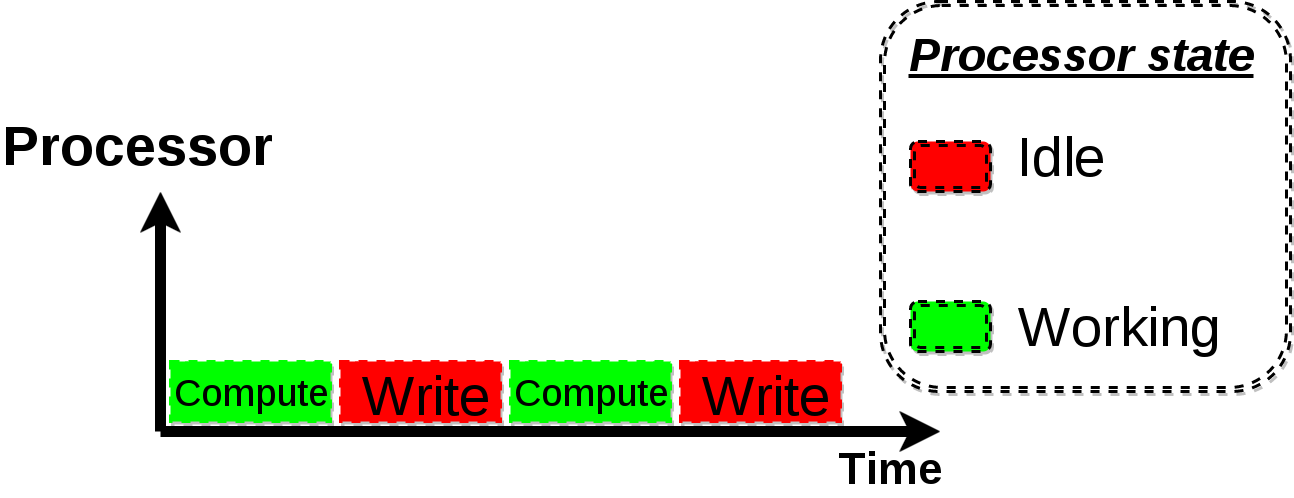
\includegraphics[width=1\textwidth, height=0.6\textheight]{images/internship_juelich_cubeRemapper_pattern.png}
		\end{figure}
	\end{frame}


%----------------------------------------
	\begin{frame}
		\frametitle{Motivation: avoid idle write time}
		\center
		\begin{figure}
			\center
			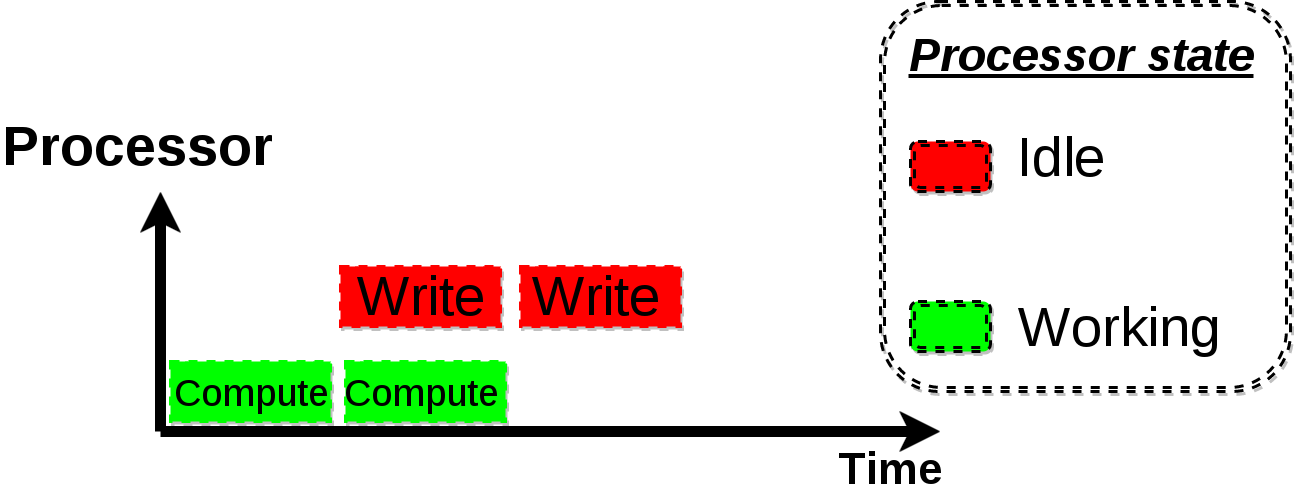
\includegraphics[width=1\textwidth, height=0.6\textheight]{images/internship_juelich_cubeRemapper_pattern_ideal.png}
		\end{figure}
		
		\pause
		\begin{block}{Target software optimization}
			The \toolTargetSoftware
		\end{block}

	\end{frame}


%----------------------------------------
\AtBeginSection[]
{
	\begin{frame}
		\frametitle{Table of Contents}
		\tableofcontents[currentsection]
	\end{frame}
}

\section*{Table of Contents}
\begin{frame}[fragile]
	\frametitle{Table of Contents}
	\tableofcontents
\end{frame}


% ----------------------------------------------------------------------------------------
%	Environment and objective
% ----------------------------------------------------------------------------------------
\section{Basis of the custom solution}
	\subsection{The POSIX-based \notationaio\space}
		\begin{frame}
			\frametitle{The POSIX-based \notationaio\space library (\notationaioShort.h)}
			\center
			\begin{tabular}{cl}
				\begin{tabular}{c}
					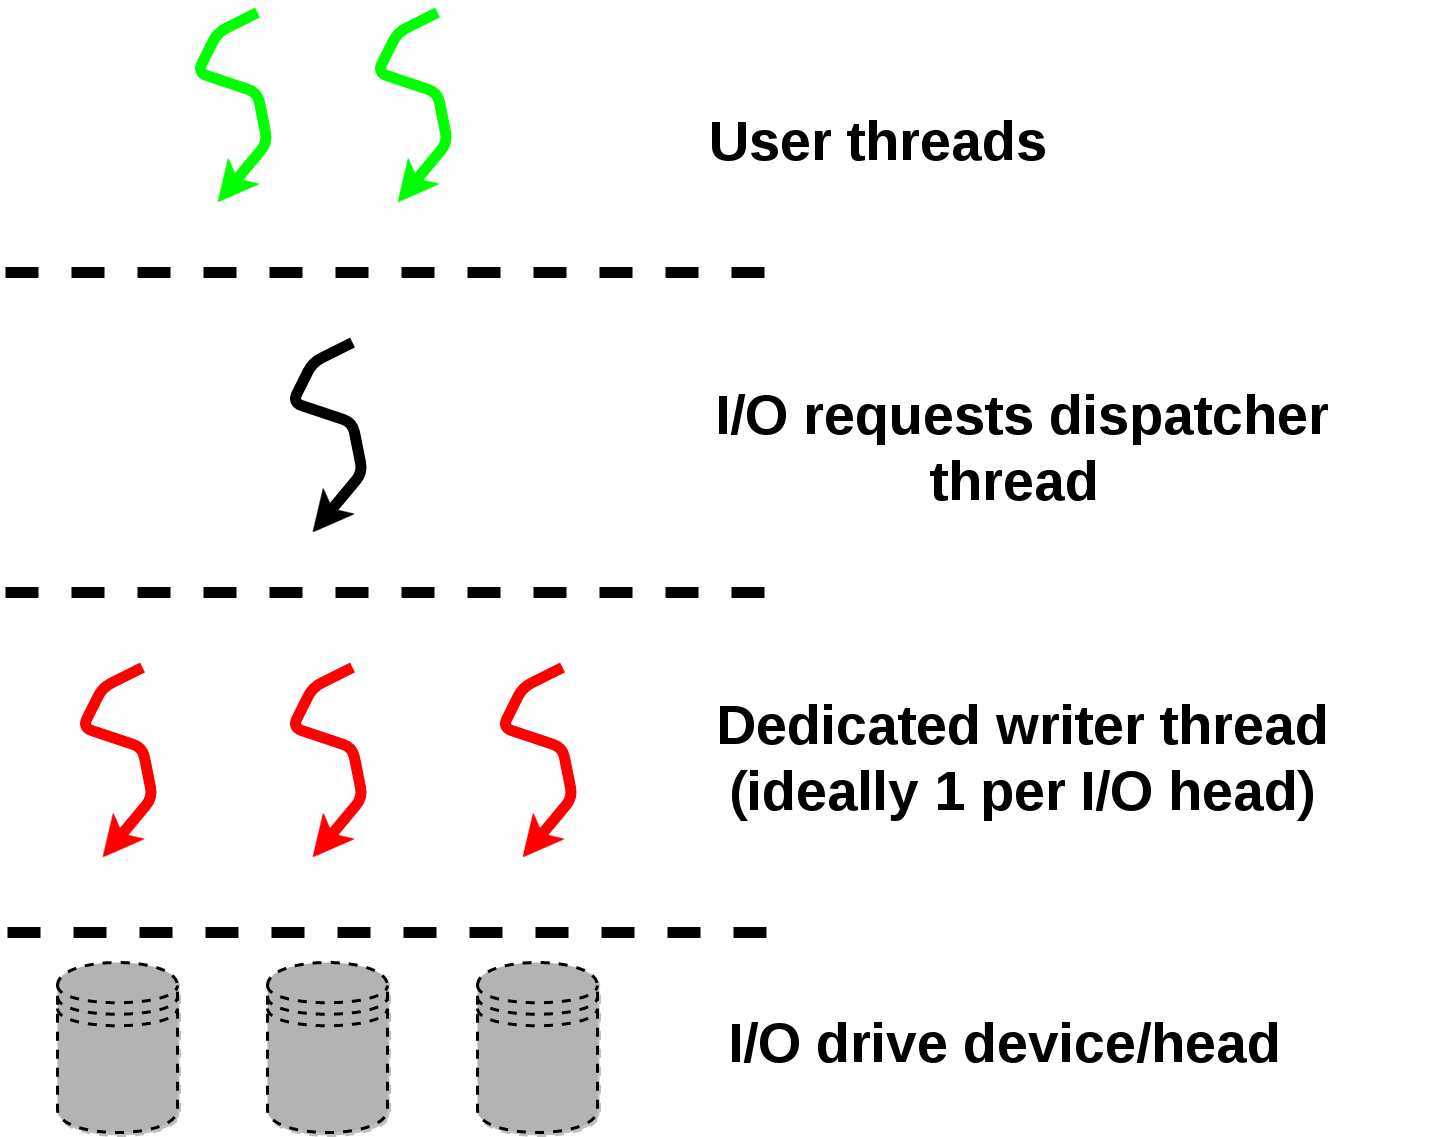
\includegraphics[width=0.42\textwidth,height=0.6\textheight]{images/internship_juelich_posixAIO_basis_slides.png}
				\end{tabular}
				&
				\begin{tabular}{l}
					\parbox{0.58\linewidth}
					{
						\begin{block}{\notationAIO\space library (\notationaioShort.h)}
							\begin{itemize}
								\item POSIX standard library
								\item Distributed on most UNIX OS: GNU-Linux, MacOsX
								\item Emulated for windows
							\end{itemize}
						\end{block}
					}
				\end{tabular}
			\end{tabular}\\
		\end{frame}


%----------------------------------------
		\begin{frame}
			\frametitle{The POSIX-based \notationaio\space library (\notationaioShort.h)}
			\center
			\begin{tabular}{cl}  
				\begin{tabular}{c}
					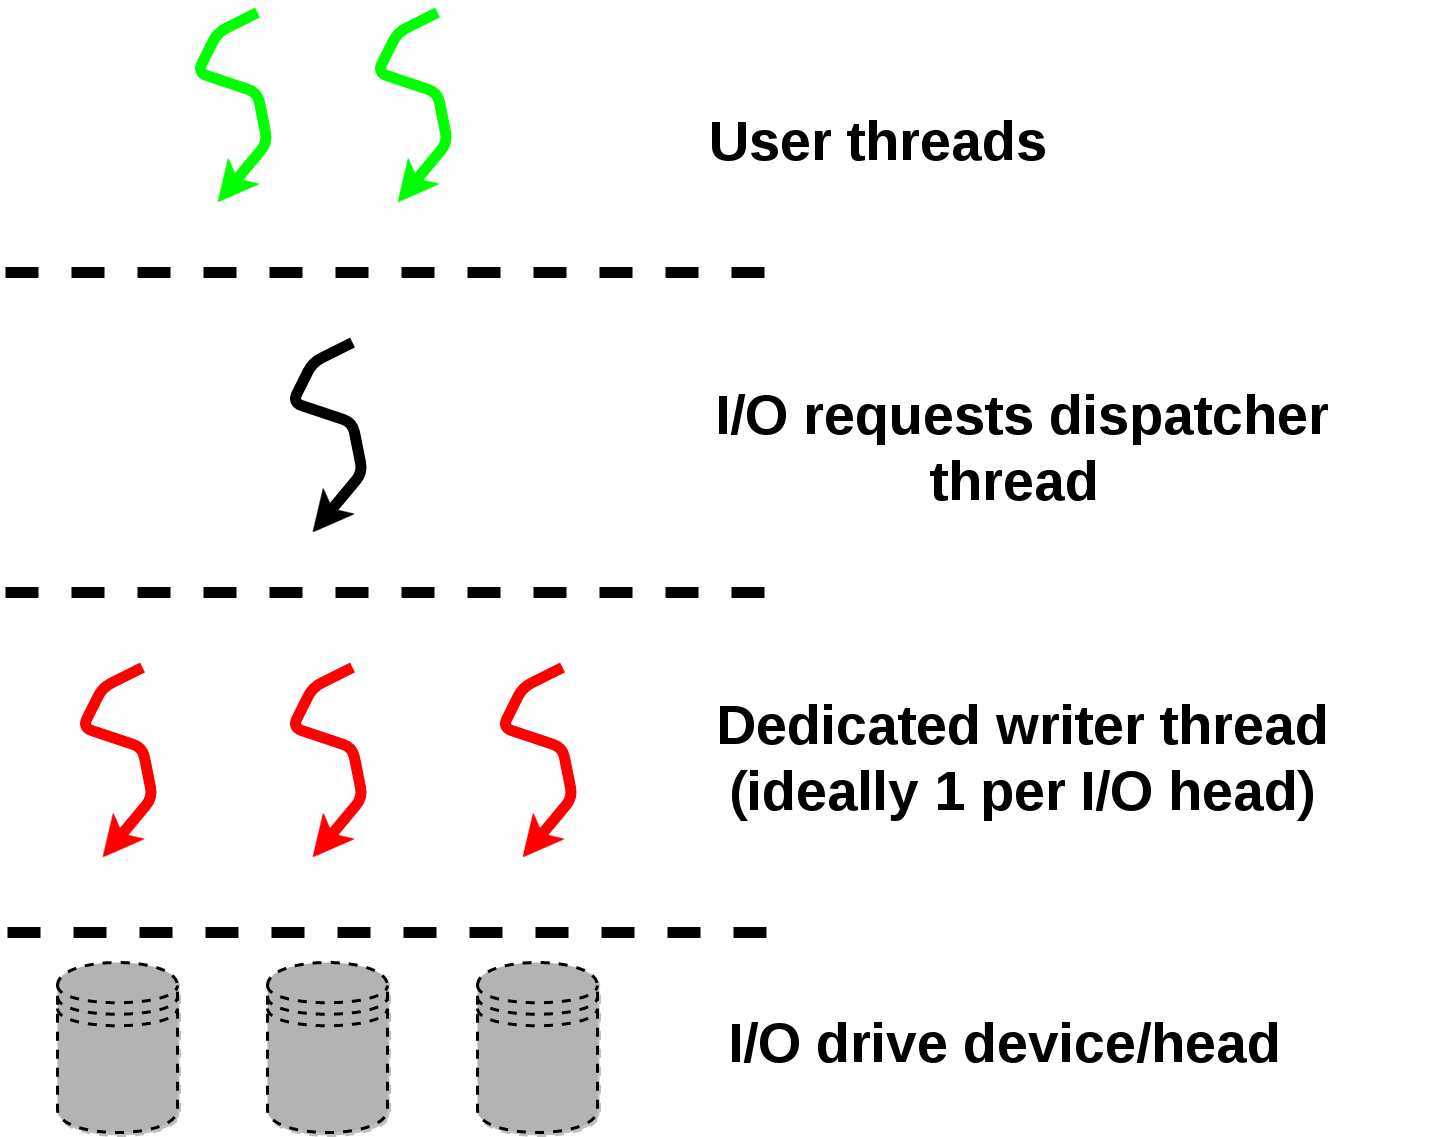
\includegraphics[width=0.42\textwidth,height=0.6\textheight]{images/internship_juelich_posixAIO_basis_slides.png}
				\end{tabular}
				&
				\begin{tabular}{l}
					\parbox{0.58\linewidth}
					{
						\begin{block}{Limitations of the \notationaioShort.h}
							\begin{itemize}
								\item Memory footprint might explode $\Rightarrow$ RAM swap
								\pause
								\item Possible contention on I/O\\ device
							\end{itemize}
						\end{block}
					}
				\end{tabular}
			\end{tabular}\\
		\end{frame}


%----------------------------------------
		\begin{frame}
			\frametitle{The POSIX-based \notationaio\space library (\notationaioShort.h)}
			\center
			\begin{tabular}{cl}
				\begin{tabular}{c}
					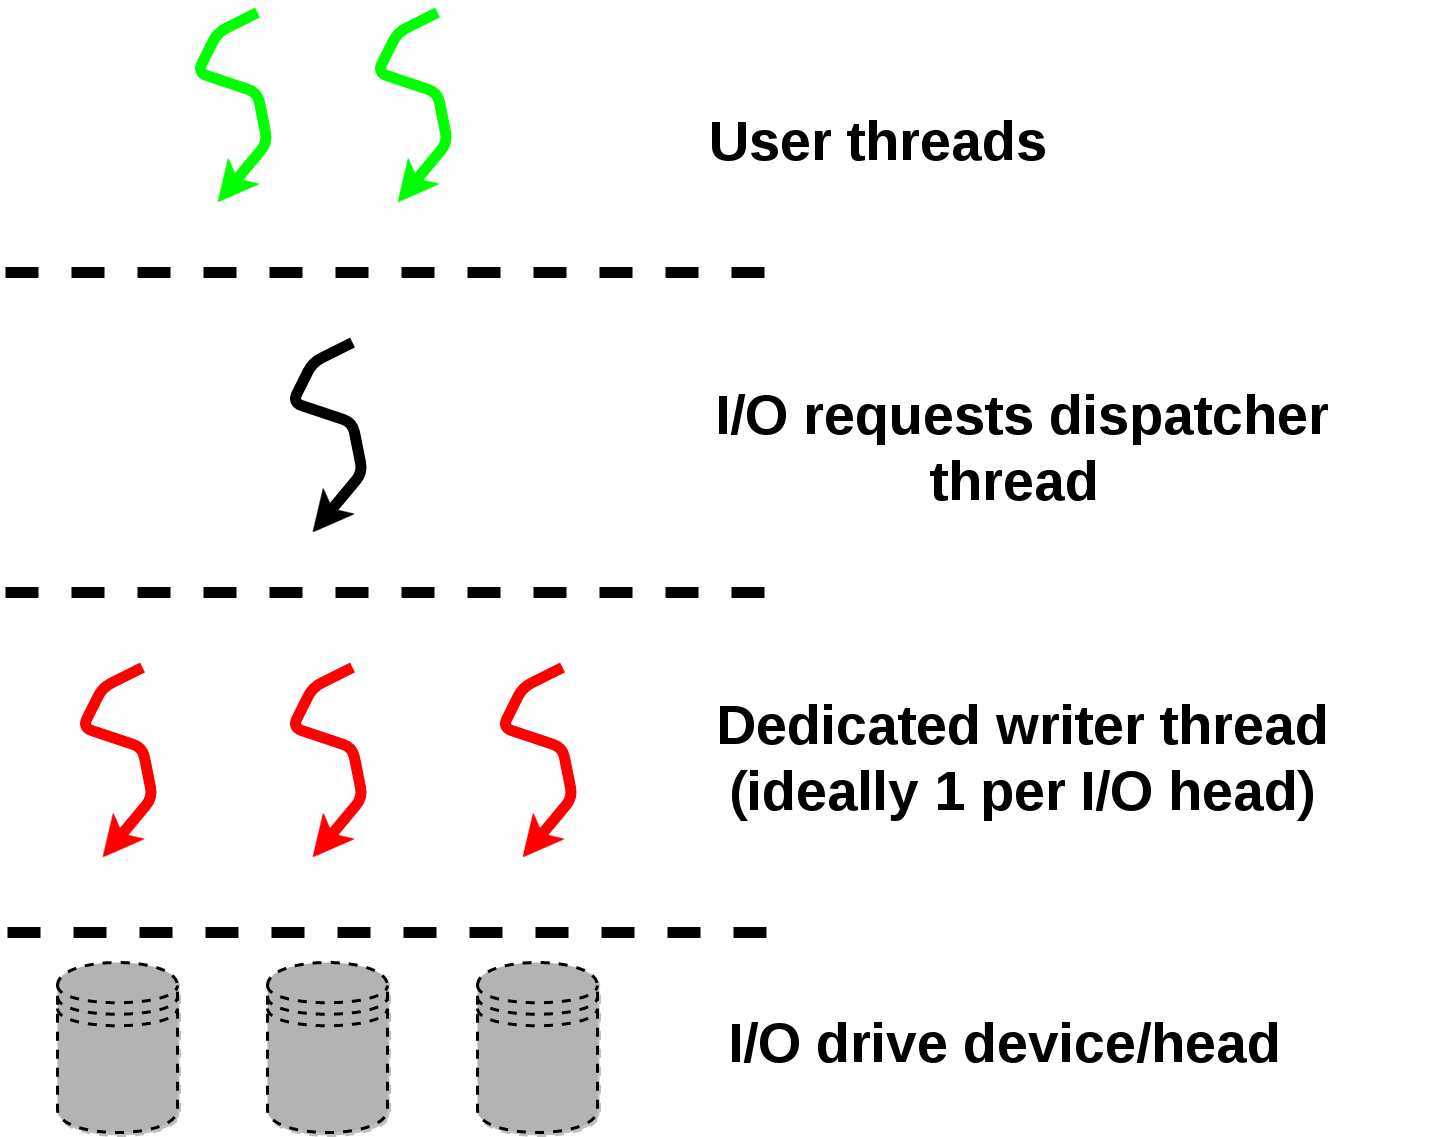
\includegraphics[width=0.42\textwidth,height=0.6\textheight]{images/internship_juelich_posixAIO_basis_slides.png}
				\end{tabular}
				&
				\begin{tabular}{l}
					\parbox{0.58\linewidth}
					{
						\begin{block}{Why this choice?}
							\begin{itemize}
								\item Minimize the engineering effort
								\pause
								\item Tuned to fit:
									\begin{itemize}
										\item I/O access pattern
										\item Hardware specification
									\end{itemize}
							\end{itemize}
						\end{block}
					}
				\end{tabular}
			\end{tabular}\\
		\end{frame}


%----------------------------------------
		\defverbatim[colored]
		\lst
		{
			\begin{lstlisting}[tabsize=2,basicstyle=\ttfamily]
void mainCubeRemapper
{
    Cube* inCube = new Cube(input);

    for (int i=0; i<nbMetric;++i)
    {
        File* result = openFile("w");
        <@\textcolor{green}{compute(inCube, i, \&bufer);}@>
        <@\textcolor{red}{write(buffer, result);}@>
    }
}
			\end{lstlisting}
		}

		\begin{frame}
			\frametitle{The \toolTargetSoftware}
			\begin{columns}[T]
				\begin{column}{.5\textwidth}
					\begin{minipage}[b]{0.6\textwidth}%
						\lst
					\end{minipage}
				\end{column}
				\begin{column}{.5\textwidth}
				\end{column}
			\end{columns}
		\end{frame}


%----------------------------------------
		\defverbatim[colored]
		\lst
		{
			\begin{lstlisting}[tabsize=2,basicstyle=\ttfamily]
void mainCubeRemapper
{
    Cube* inCube = new Cube(input);

    for (int i=0; i<nbMetric;++i)
    {
        File* result = openFile("w");
        compute(inCube, i, &bufer);
        <@\textcolor{red}{asynchronous\_write(buffer, result);}@>
    }
}
			\end{lstlisting}
		}

		\begin{frame}
			\frametitle{The \toolTargetSoftware\space (\notationaio\space version)}
			\begin{columns}[T]
				\begin{column}{.5\textwidth}
					\begin{minipage}[b]{0.6\textwidth}%
						\lst
					\end{minipage}
				\end{column}
				\begin{column}{.5\textwidth}
				\end{column}
			\end{columns}
		\end{frame}


%----------------------------------------
		\defverbatim[colored]
		\lst
		{
			\begin{lstlisting}[tabsize=2,basicstyle=\ttfamily]
void mainCubeRemapper
{
    Cube* inCube = new Cube(input);

    for (int i=0; i<nbMetric;++i)
    {
        File* result = openFile("w");
        compute(inCube, i, &bufer);
        <@\textcolor{red}{asynchronous\_write(buffer, result);}@>
    }
    <@\textcolor{red}{wait\_asynchronous\_write();}@>
}
			\end{lstlisting}
		}


		\begin{frame}
			\setbeamercovered{invisible}				% Used to make the "pause" invisible before it is printed
			\frametitle{The \toolTargetSoftware\space (\notationaio\space version)}
			\begin{columns}[T]
				\begin{column}{.5\textwidth}
					\begin{minipage}[b]{0.6\textwidth}%
						\lst
					\end{minipage}
				\end{column}


				\begin{column}{.5\textwidth}
					\pause
					\begin{block}{The asynchronous choice}
						\begin{itemize}
							\item Reduce processor stall
							\pause
							\item Benefit from data distribution
						\end{itemize}
					\end{block}
				\end{column}
			\end{columns}
		\end{frame}


% ----------------------------------------------------------------------------------------
%	The asynchronous-writing approach
% ----------------------------------------------------------------------------------------
\section{Modelling the solution's gain}
		\begin{frame}
			\frametitle{Current synchronous model}
			\center
			\begin{tabular}{cl}  
				\begin{tabular}{c}
					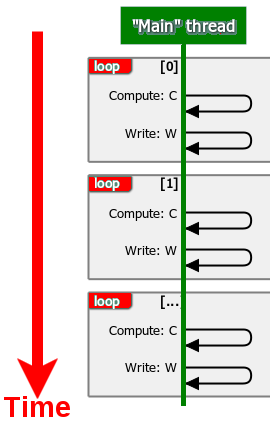
\includegraphics[width=0.4\textwidth]{images/internshipJulich_model_0-IO-simple.png}
				\end{tabular}
				&
				\begin{tabular}{l}
					\parbox{0.6\linewidth}
					{
						\begin{block}{Synchronous I/O model}
							\begin{itemize}
								\item Current version of the  \toolTargetSoftware
								\item Benchmark for the study
								\item $\mathcolorbox{yellow}{T_{synchronous} = n * (C + W)}$
							\end{itemize}
						\end{block}
					}
				\end{tabular}
			\end{tabular}\\
		\end{frame}


%----------------------------------------
		\begin{frame}
			\frametitle{Simplified \notationaio\space model}
			\center
			\begin{tabular}{cl}  
				\begin{tabular}{c}
					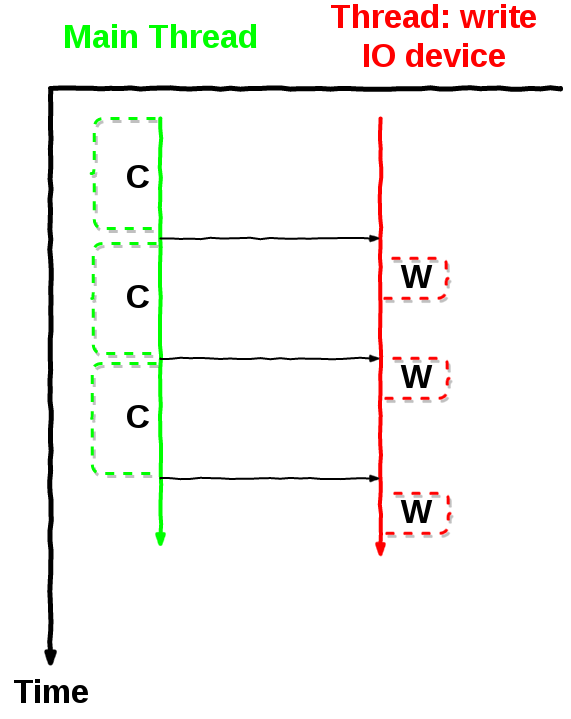
\includegraphics[width=0.4\textwidth]{images/internshipJulich_model_0-AIO-simple.png}
				\end{tabular}
				&
				\begin{tabular}{l}
					\parbox{0.6\linewidth}
					{
						\begin{block}{\notationAIO\space model}
							Assumptions:
							\begin{itemize}
								\item Constant writing time W of each buffer
								\item Constant computation time C
							\end{itemize}
						\end{block}
					}
				\end{tabular}
			\end{tabular}\\
		\end{frame}


%----------------------------------------
		\begin{frame}
			\frametitle{Simplified \notationaio\space model}
			\center
			\begin{tabular}{cl}  
				\begin{tabular}{c}
					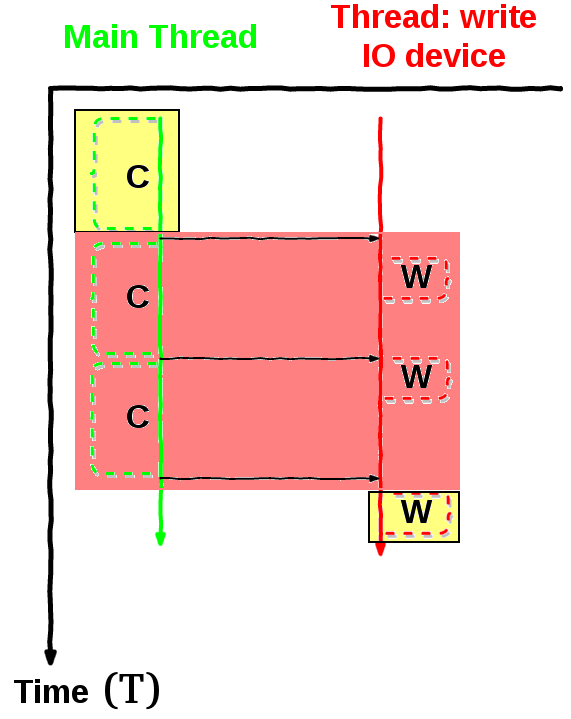
\includegraphics[width=0.39\textwidth,height=0.7\textheight]{images/internshipJulich_model_0-AIO-spotFirsC-lastW.png}
				\end{tabular}
				&
				\begin{tabular}{l}
					\parbox{0.61\linewidth}
					{
						\begin{block}{\notationAIO\space model}
							$T = \mathcolorbox{yellow}{C} + \mathcolorbox{yellow}{W} + \mathcolorbox{salmon}{(n-1) * max(C, W)}$ \\\\
							\pause
							$T \stackrel{\text{if C << W}}{\approx} n * W + C$ \\\\
							$T \stackrel{\text{if C >> W}}{\approx} n * C + W$
						\end{block}
					}
				\end{tabular}
			\end{tabular}\\
		\end{frame}


%----------------------------------------
		\begin{frame}
			\frametitle{Simplified model assessment}
			\center
			\begin{figure}[!h]
				\centering
				\begin{subfigure}[b]{0.48\textwidth}
					\centering
					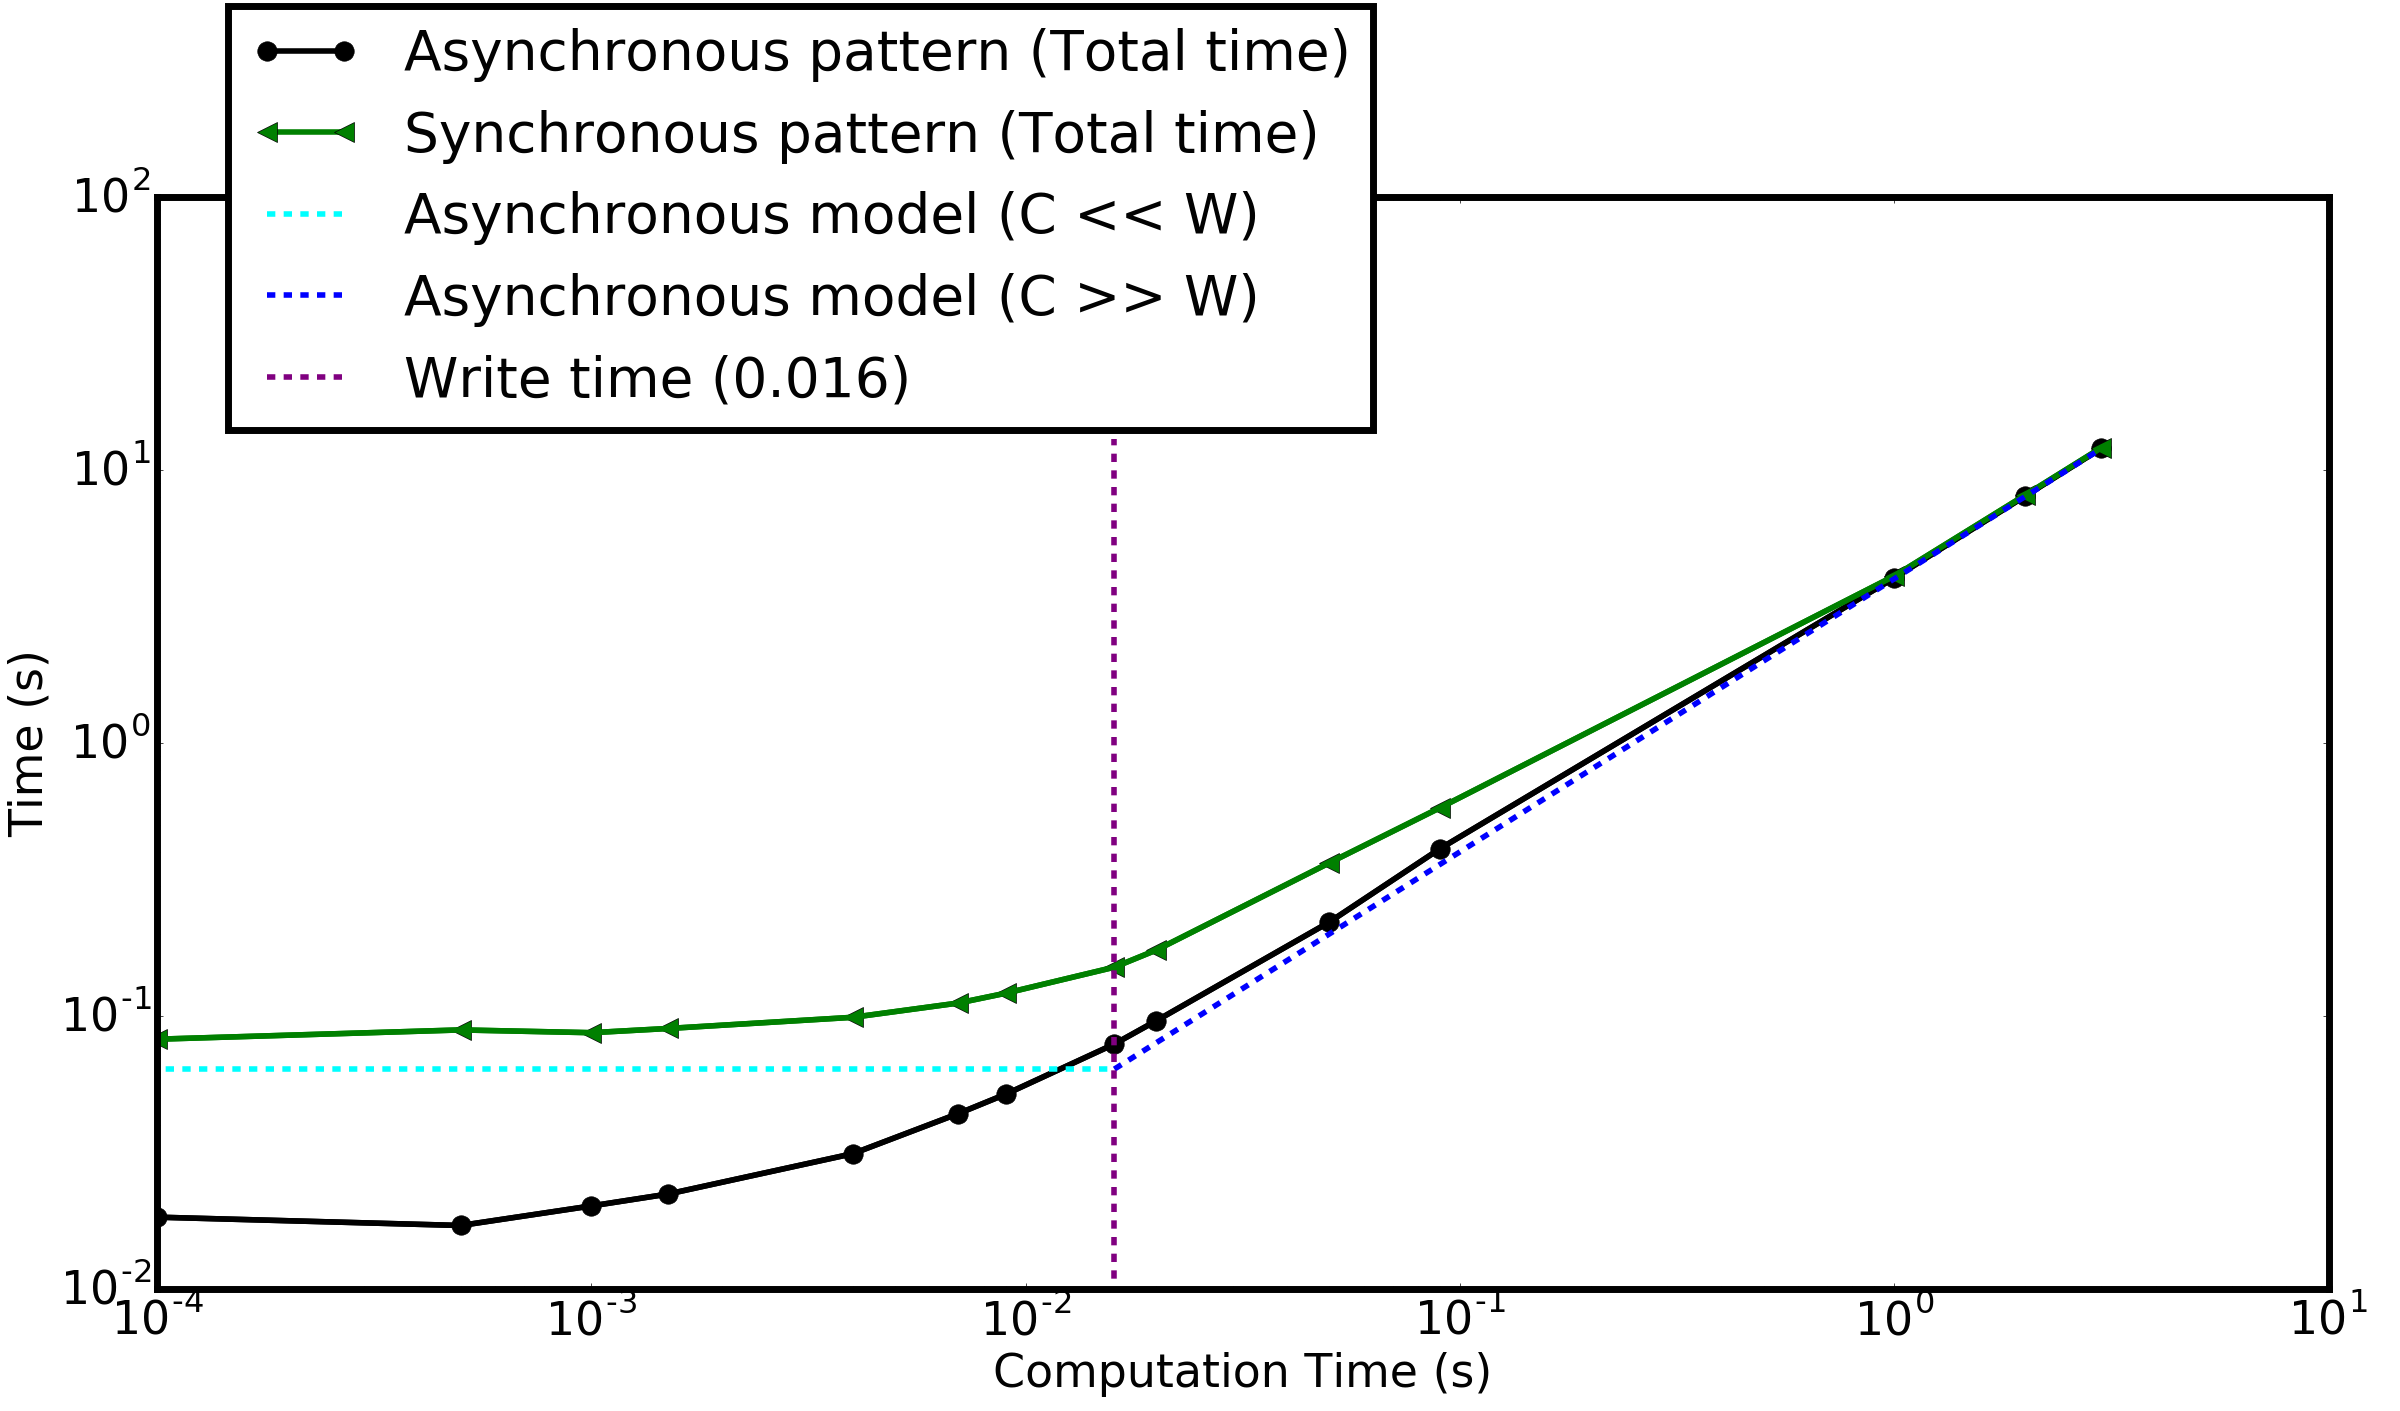
\includegraphics[width=\textwidth]{images/model0_workstation_8core_logScale.png}
					\caption[]%
					{{\small \targetPlatformLaptop}}
				\end{subfigure}
				\hfill
				\begin{subfigure}[b]{0.475\textwidth}  
					\centering 
					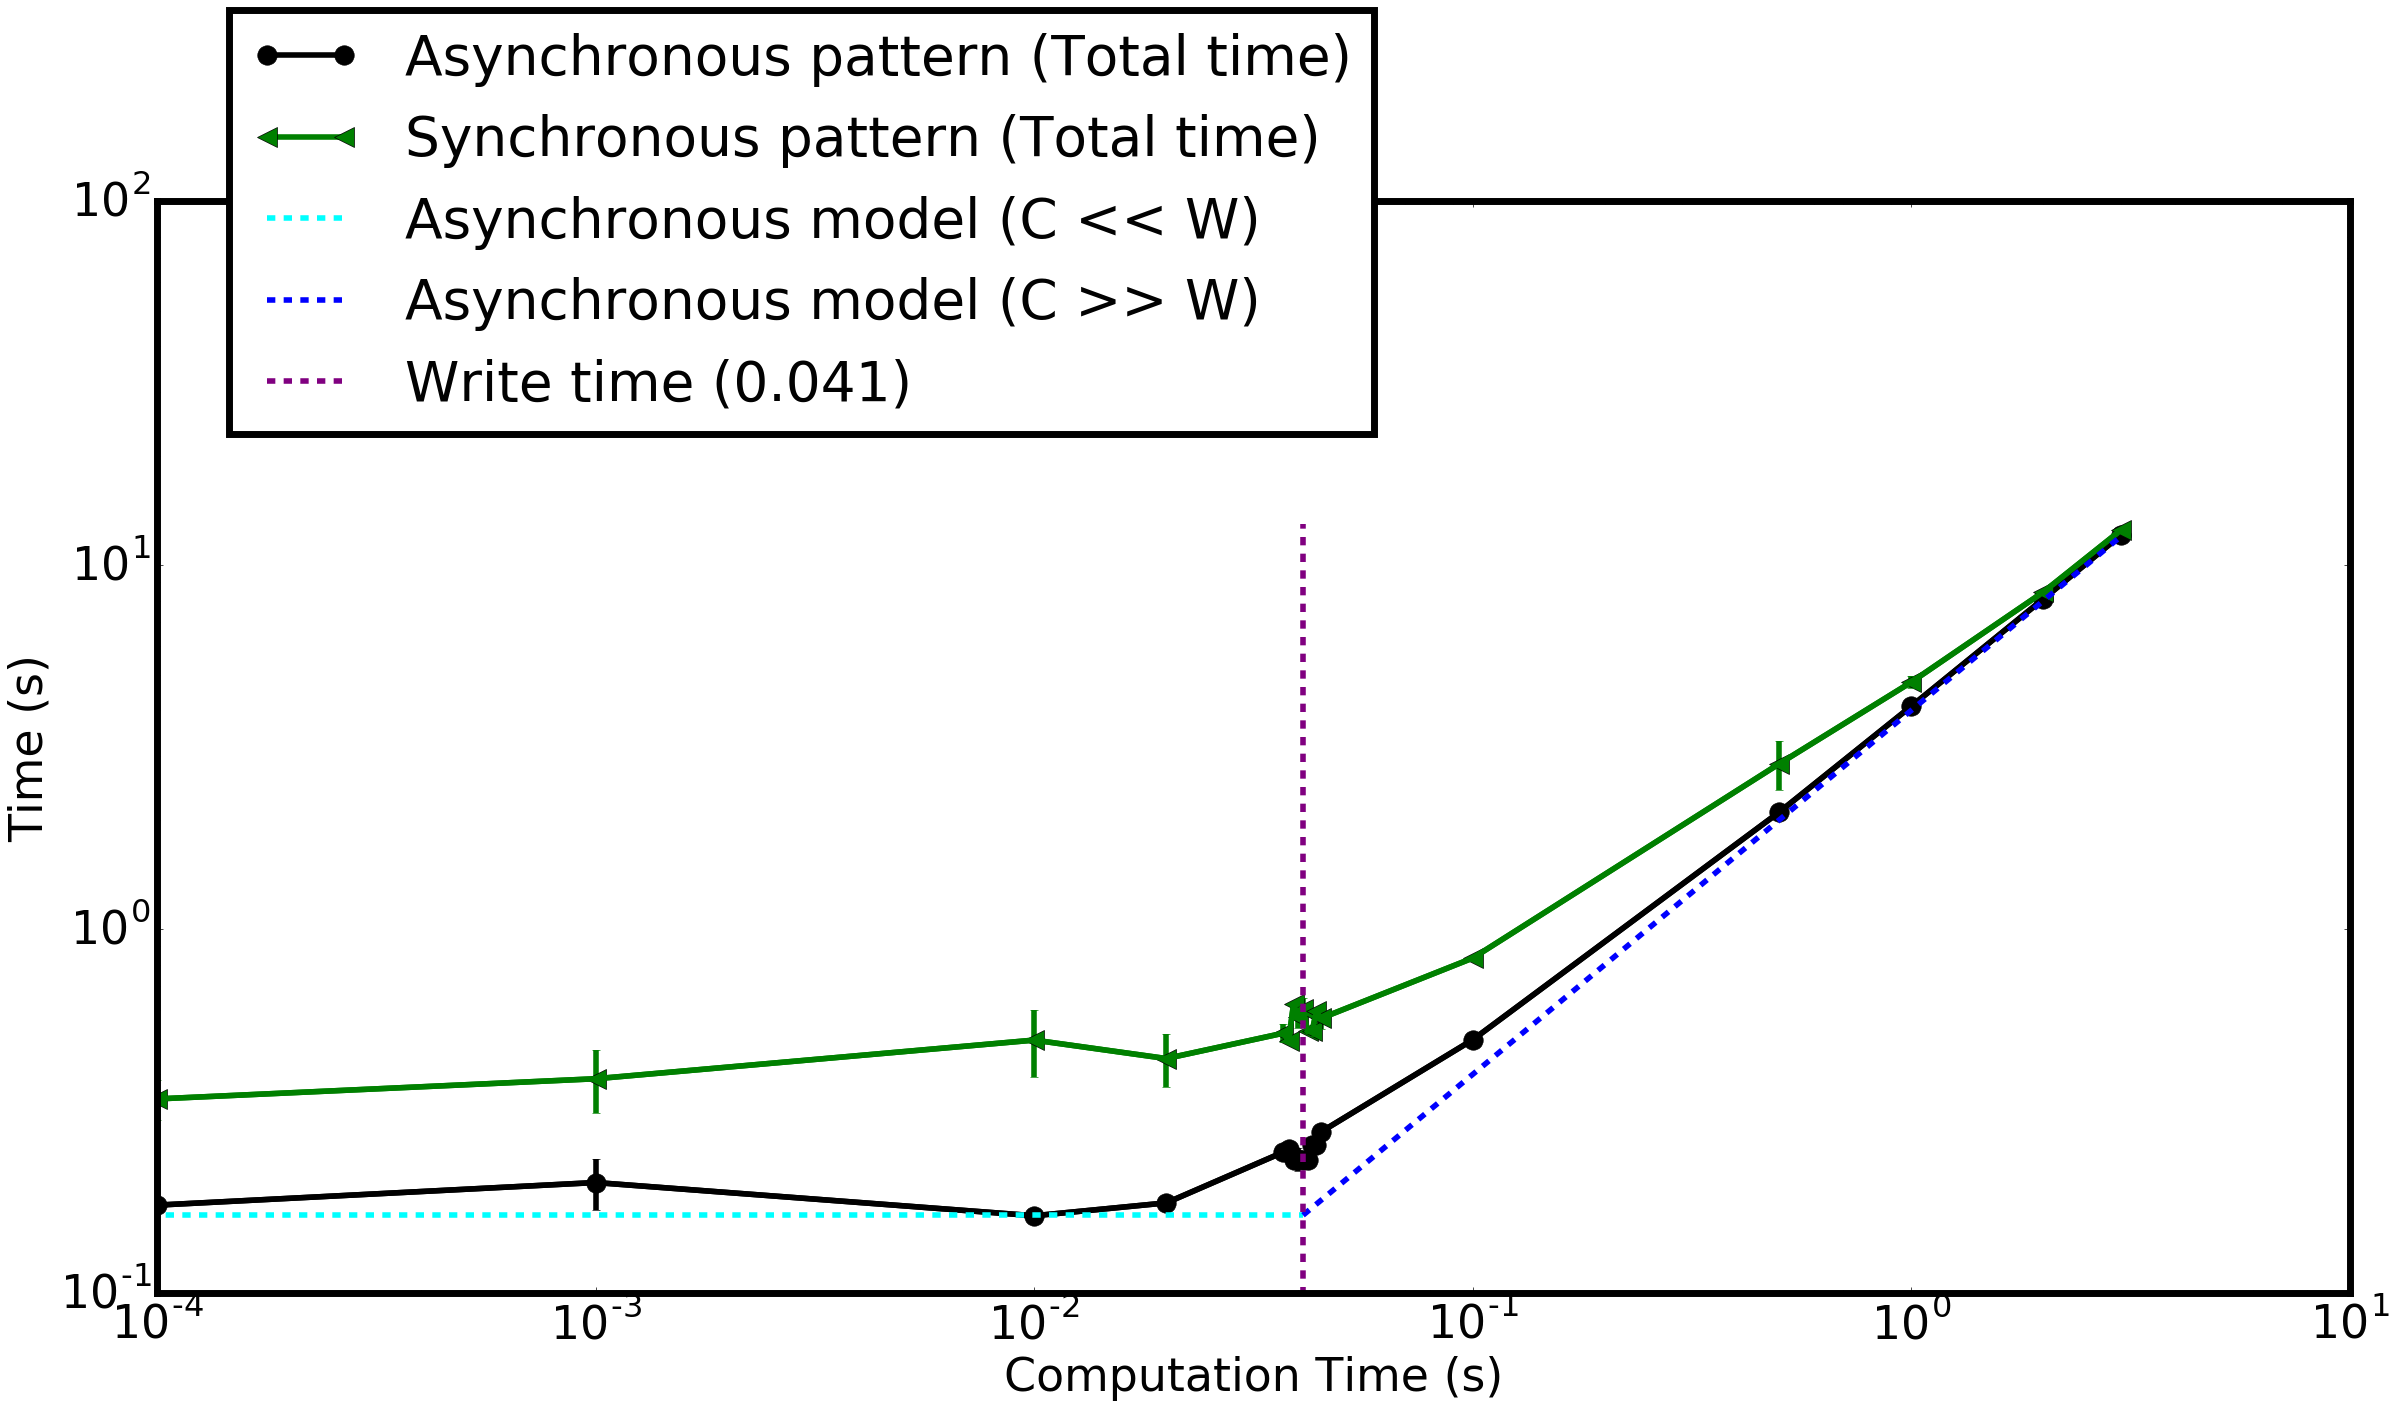
\includegraphics[width=\textwidth]{images/model0_hpc_2Proc_1IoDevice_logScale.png}
					\caption[]%
					{{\small \targetPlatformHpc}}
				\end{subfigure}
			\end{figure}

			\begin{block}{}
			\begin{itemize}
				\item Experimental improvement brought by \notationaio
				\item Maximum improvement for $C \sim W$
				\pause
				\item Potential inaccuracy $\Rightarrow$ model 2 (\emph{cf} report)
			\end{itemize}

			
			
			

			\end{block}
		\end{frame}


%----------------------------------------
		\begin{frame}
			\frametitle{Multiple I/O devices: case $C >> W$}
			\center
			\begin{tabular}{cl}  
				\begin{tabular}{c}
					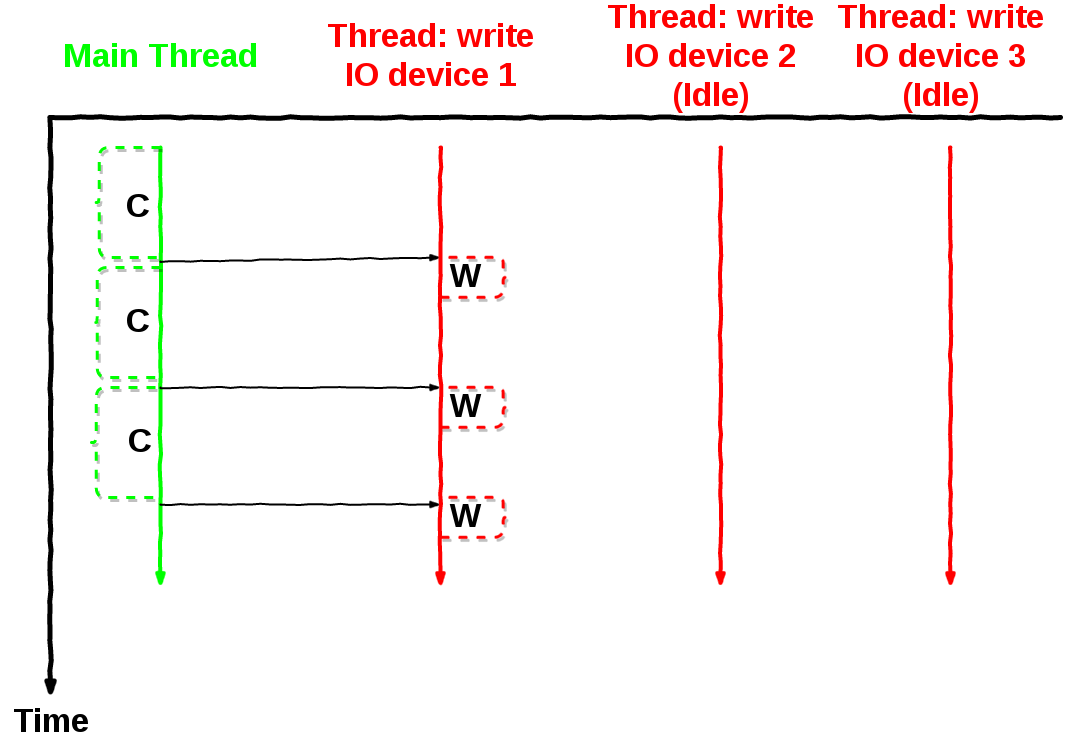
\includegraphics[width=0.5\textwidth,height=0.7\textheight]{images/internshipJulich_AIO-multipleIoDevice_CBiggerThanW.png}
				\end{tabular}
				&
				\begin{tabular}{l}
					\parbox{0.6\linewidth}
					{
						\begin{block}{Theoretical model}
							\begin{itemize}
%								\item No linear dependency with $W$
								\item $\mathcolorbox{yellow}{T(N_{io})\stackrel{\text{if C >> W}}{\approx} n * C + W}$
								\pause
								\item Useless additional \notationIO
							\end{itemize}
						\end{block}
					}
				\end{tabular}
			\end{tabular}\\
		\end{frame}


%----------------------------------------
		\begin{frame}
			\frametitle{Multiple I/O devices: case $C << W$}
			\center
			\begin{tabular}{cl}  
				\begin{tabular}{c}
					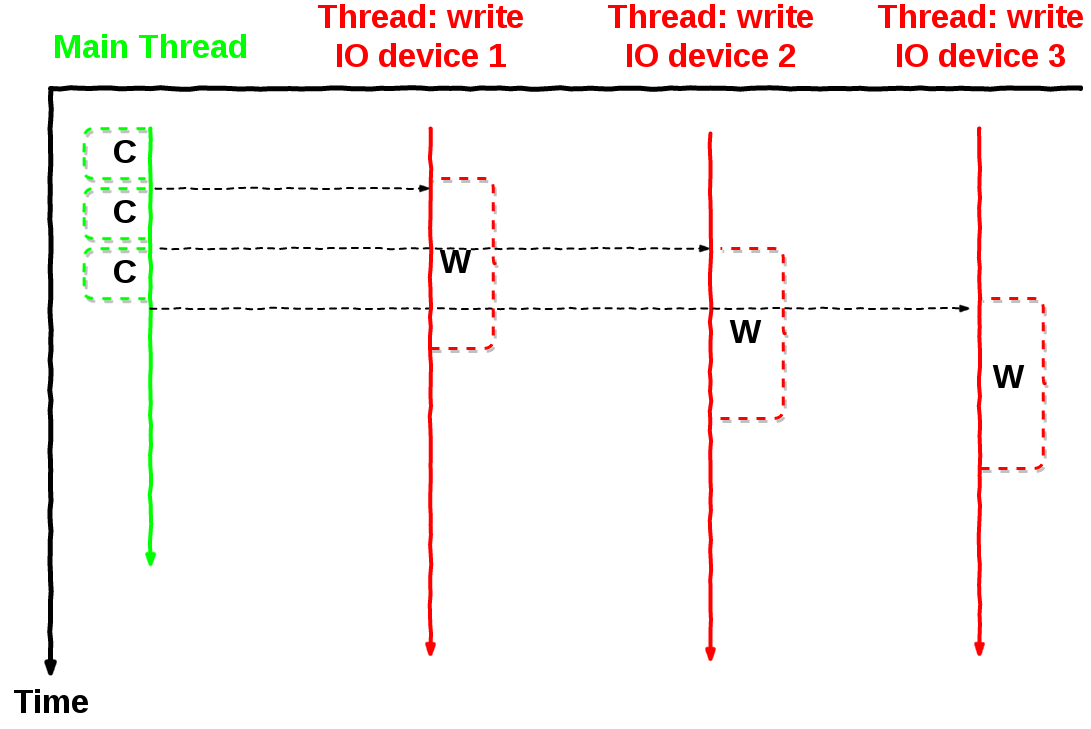
\includegraphics[width=0.42\textwidth,height=0.65\textheight]{images/internshipJulich_AIO-multipleIoDevice_CSmallerThanW.png}
				\end{tabular}
				&
				\begin{tabular}{l}
					\parbox{0.7\linewidth}
					{
						\begin{block}{Theoretical model}
							{\scriptsize $T(N_{io}) \stackrel{\text{if C << W}}{\approx}					C + W + (n-1) * max(\frac{W}{N_{io}}, C)$}\\\\
							{\scriptsize $T(N_{io}) \stackrel{\text{if C << }\frac{W}{N_{io}} }{\approx}	C + W + (n-1) * \frac{W}{N_{io}}$}
						\end{block}
					}
				\end{tabular}
			\end{tabular}\\
		\end{frame}


%----------------------------------------
		\begin{frame}
			\frametitle{Multiple I/O devices: case $C << W$}
			\center
			\begin{tabular}{cl}  
				\begin{tabular}{c}
					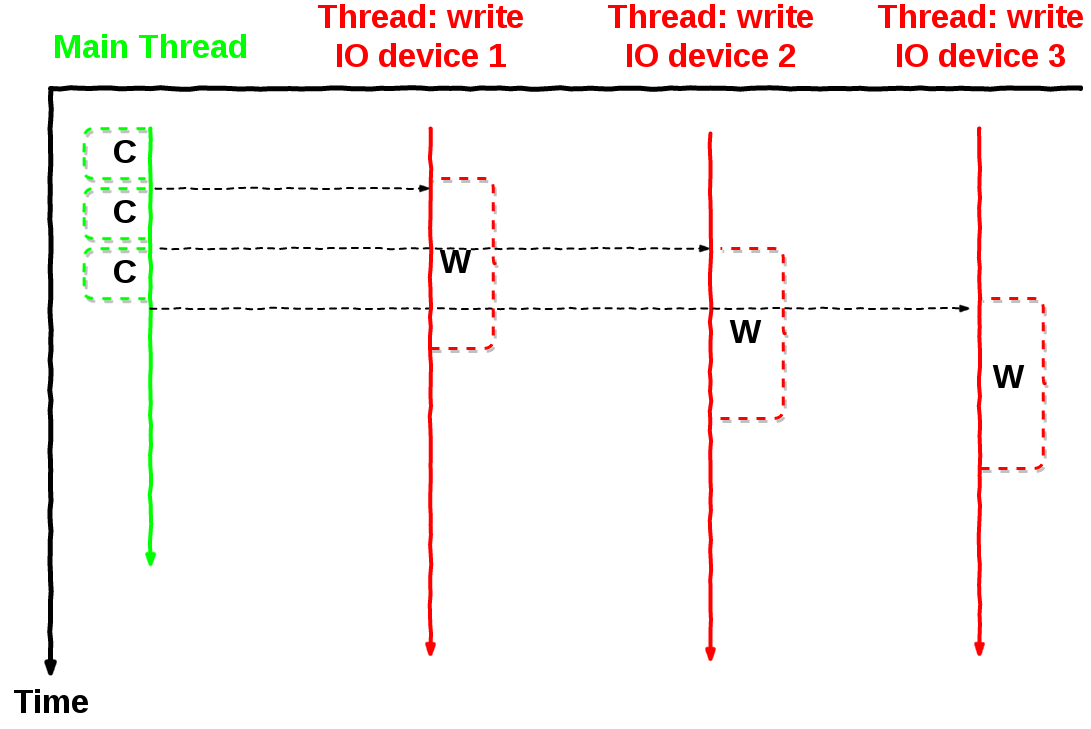
\includegraphics[width=0.42\textwidth,height=0.65\textheight]{images/internshipJulich_AIO-multipleIoDevice_CSmallerThanW.png}
				\end{tabular}
				&
				\begin{tabular}{l}
					\parbox{0.7\linewidth}
					{
						\begin{block}{Real-life execution}
							\begin{itemize}
								\item Relevant additional \notationIO
								\pause
								\item Complicated implementation
							\end{itemize}
						\end{block}
					}
				\end{tabular}
			\end{tabular}\\
		\end{frame}


% ----------------------------------------------------------------------------------------
%	The \toolTargetSoftware
% ----------------------------------------------------------------------------------------
\section{Improving the \protect\toolTargetSoftware\space}
		\begin{frame}
			\frametitle{Experimental set-up}
			\centering
			Evaluation of custom implementations of \toolTargetSoftware\space using:
			\begin{itemize}
				\item Real-life input file (\textbf{NAS parallel benchmark}):
					\begin{itemize}
						\item  $65535$ threads, $0.38$ GiB
						\item $131071$ threads, $0.62$ GiB
						\item $262143$ threads, $1.28$ GiB
					\end{itemize}
				\item Real metrics (ex: CPU time, MPI communication) from HPC execution
				\item Realistic ratio $\frac{C}{W} \equiv 2$
			\end{itemize}

		\end{frame}

%----------------------------------------
	\subsection{Basic asynchronous implementation}
		\begin{frame}
			\frametitle{Basic \notationaio\space implementation}
			\begin{figure}[!h]
				\centering
				\begin{subfigure}[b]{0.7\textwidth}
					\centering
					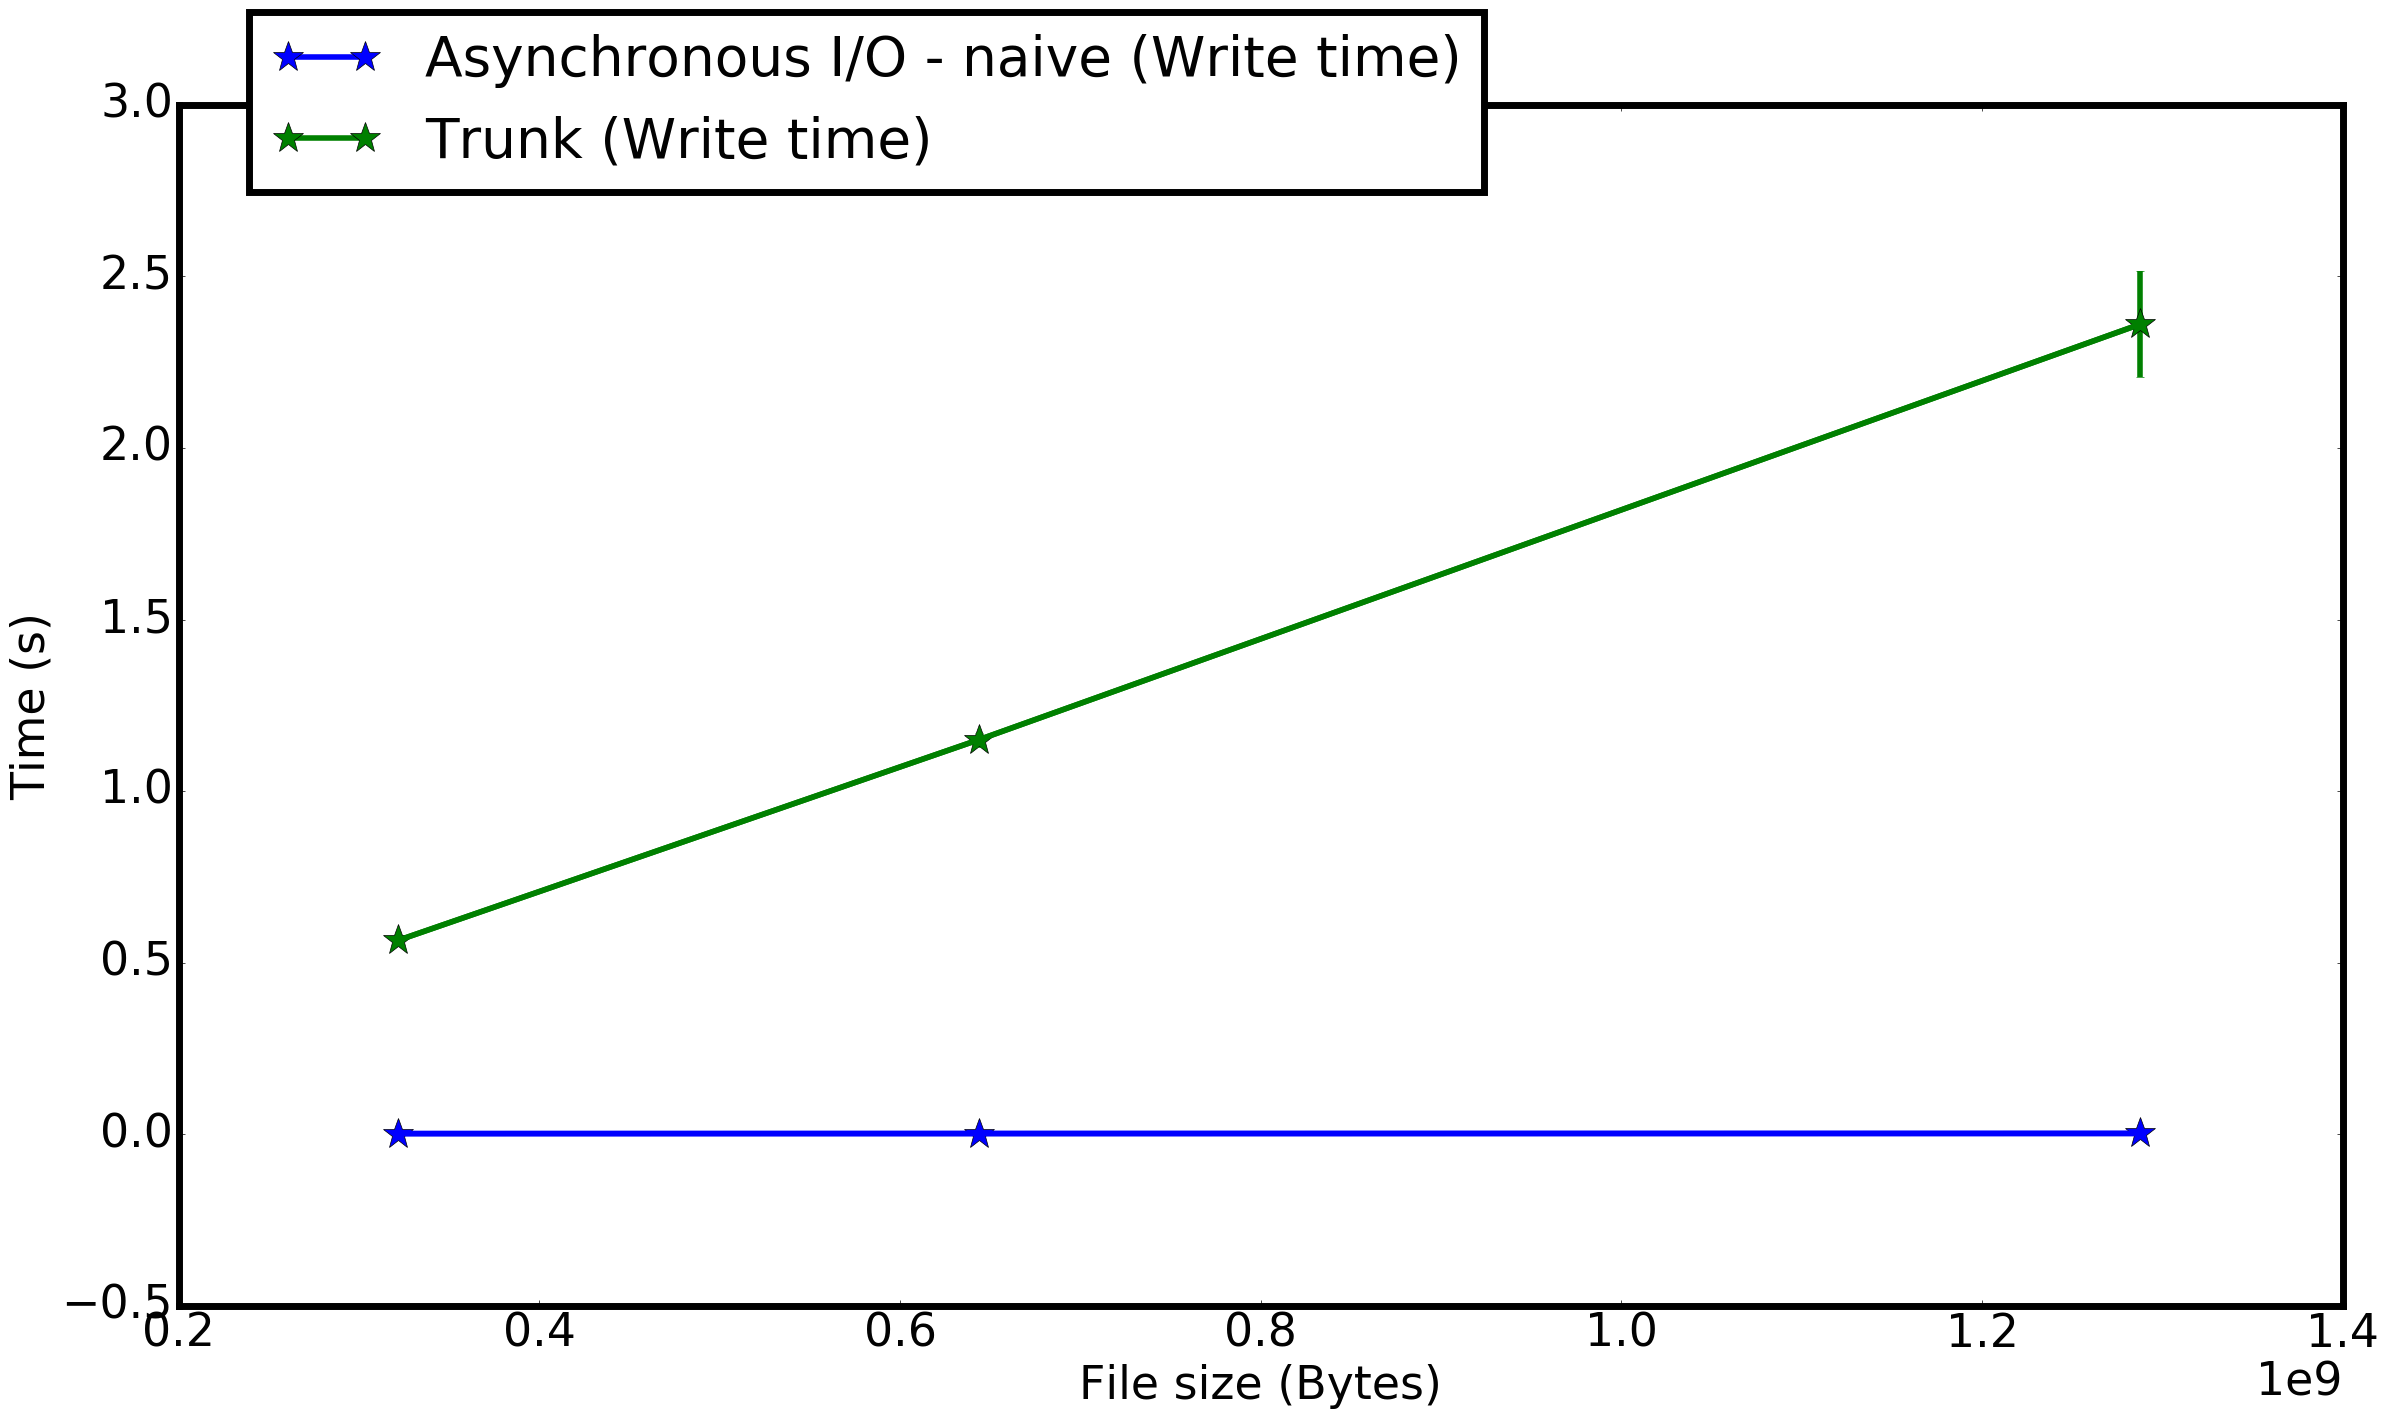
\includegraphics[width=\textwidth]{images/cubeRemapper_basicImplementation_write_hpc.png}
				\end{subfigure}
			\end{figure}

			\begin{block}{}
			\begin{itemize}
				\item Significant improvement in the \emph{"write"} time
				\item Are we done?
			\end{itemize}
			\end{block}
		\end{frame}

%----------------------------------------
		\begin{frame}
			\frametitle{Basic \notationaio\space implementation}
			\begin{figure}[!h]
				\centering
				\begin{subfigure}[b]{0.49\textwidth}
					\centering
					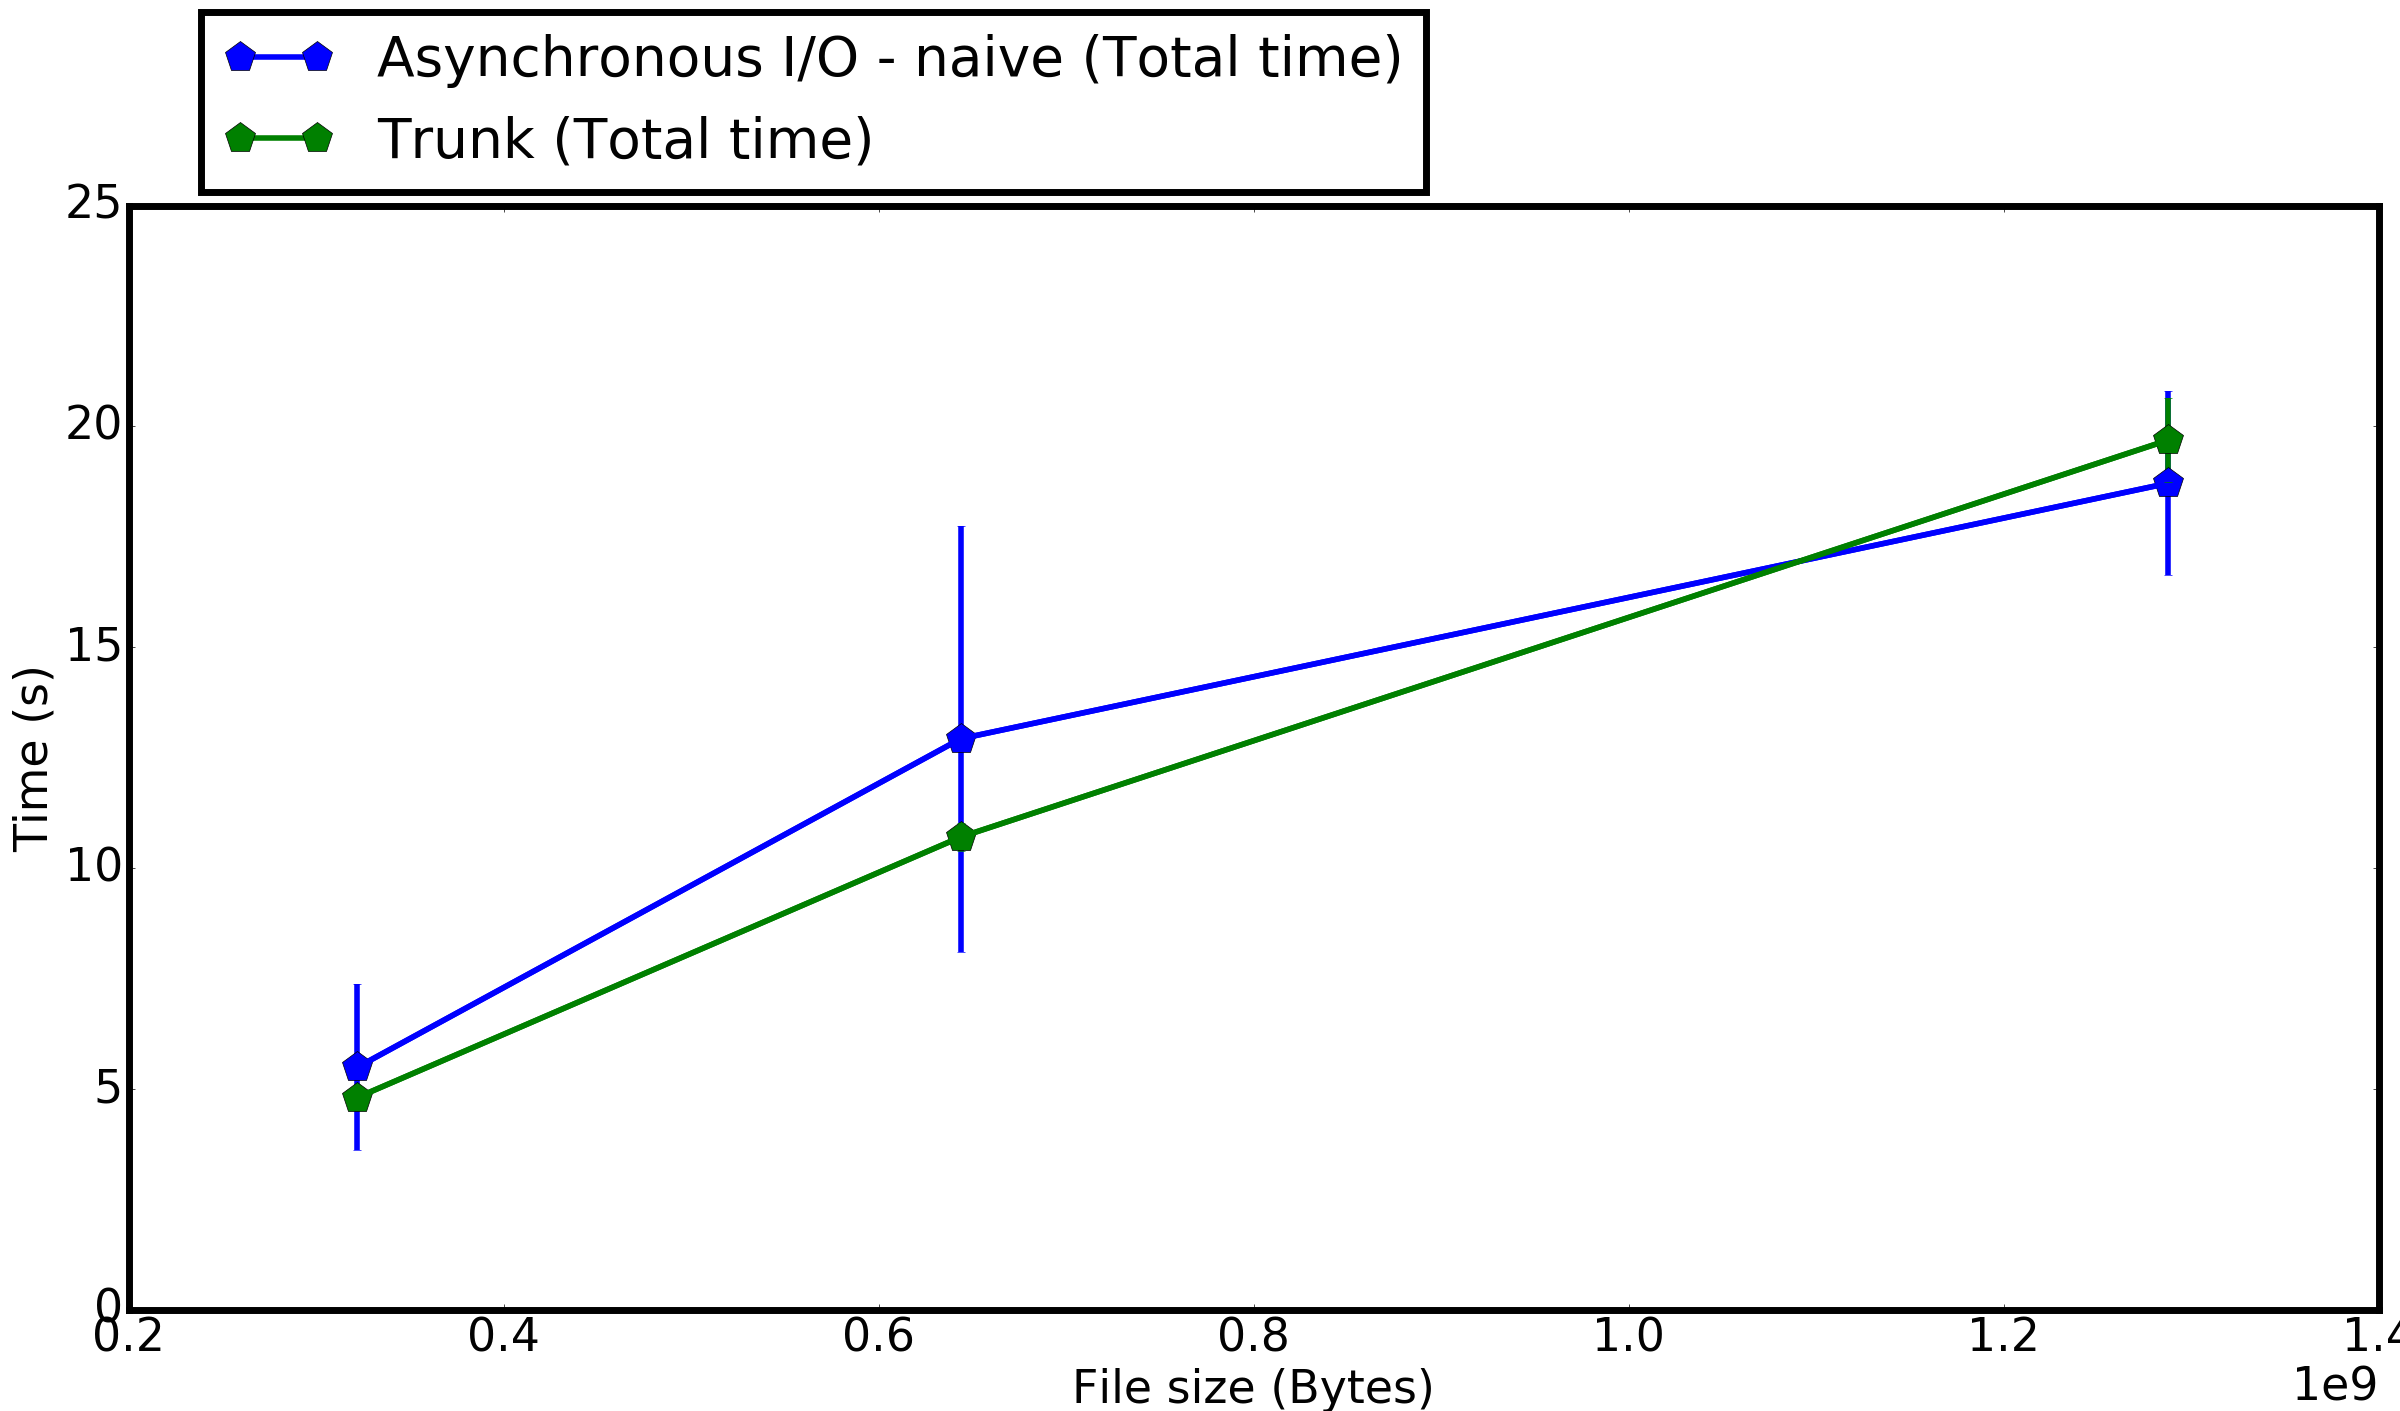
\includegraphics[width=\textwidth]{images/cubeRemapper_basicImplementation_total_hpc.png}
					\caption[\emph{"Total"} time]%
					{{\small \emph{"Total"} time}}
				\end{subfigure}
				\hfill
				\begin{subfigure}[b]{0.49\textwidth}
					\centering
					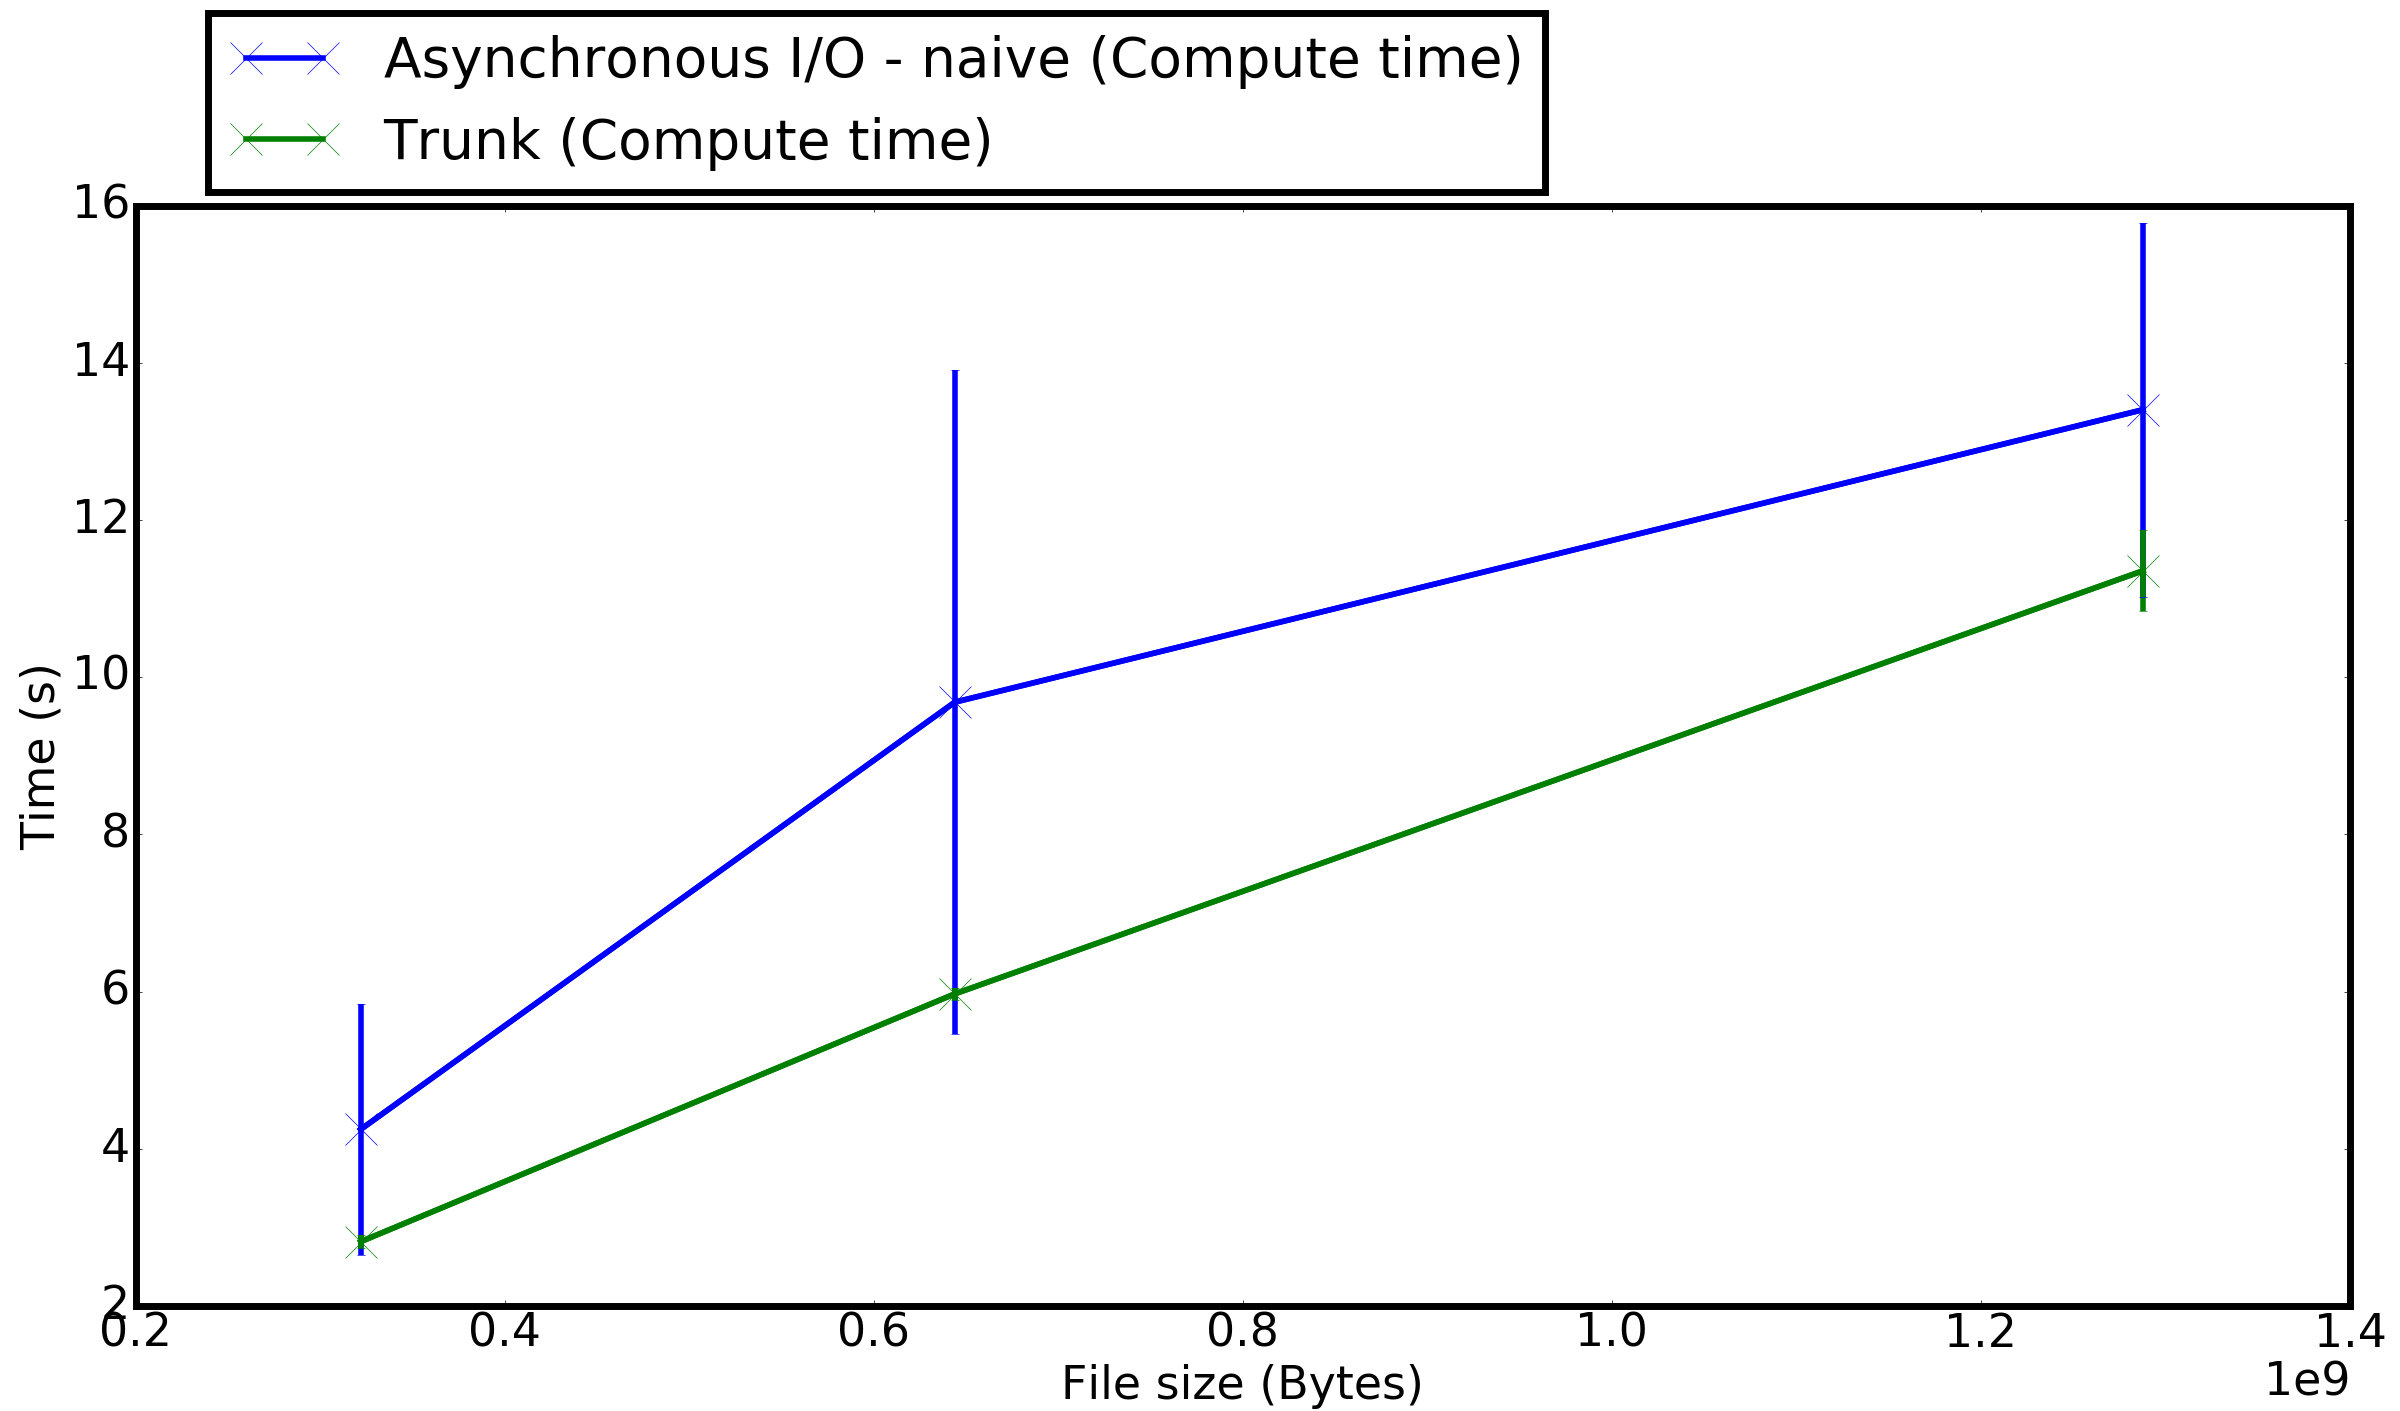
\includegraphics[width=\textwidth]{images/cubeRemapper_basicImplementation_compute_hpc.png}
					\caption[]%
					{{\small \emph{"Compute"} time}}
				\end{subfigure}
			\end{figure}

			\pause
			\begin{block}{}
			\begin{itemize}
				\item Performance loss (due to \emph{"Compute"})
				\item Uncertainty increase (due to \emph{"Compute"})
			\end{itemize}
			\end{block}
		\end{frame}


% ----------------------------------------------------------------------------------------
	\subsection{Custom enhancements}
		\begin{frame}
			\frametitle{Thread-scheduling issue}
			Threads belong to the same process $\Rightarrow$
			\begin{itemize}
				\item scheduled mostly on same CPU core (for cache proximity)
				\item Delay the \emph{"compute"} thread execution
			\end{itemize}
%			\newline
			\pause
			\textbf{Solution:} to pin threads on different CPU-cores
		\end{frame}


% ----------------------------------------------------------------------------------------
		\begin{frame}
			\frametitle{Thread scheduling solution: pin threads}
			\center
			\begin{figure}[!h]
				\centering
				\begin{subfigure}[b]{0.73\textwidth}
					\centering
					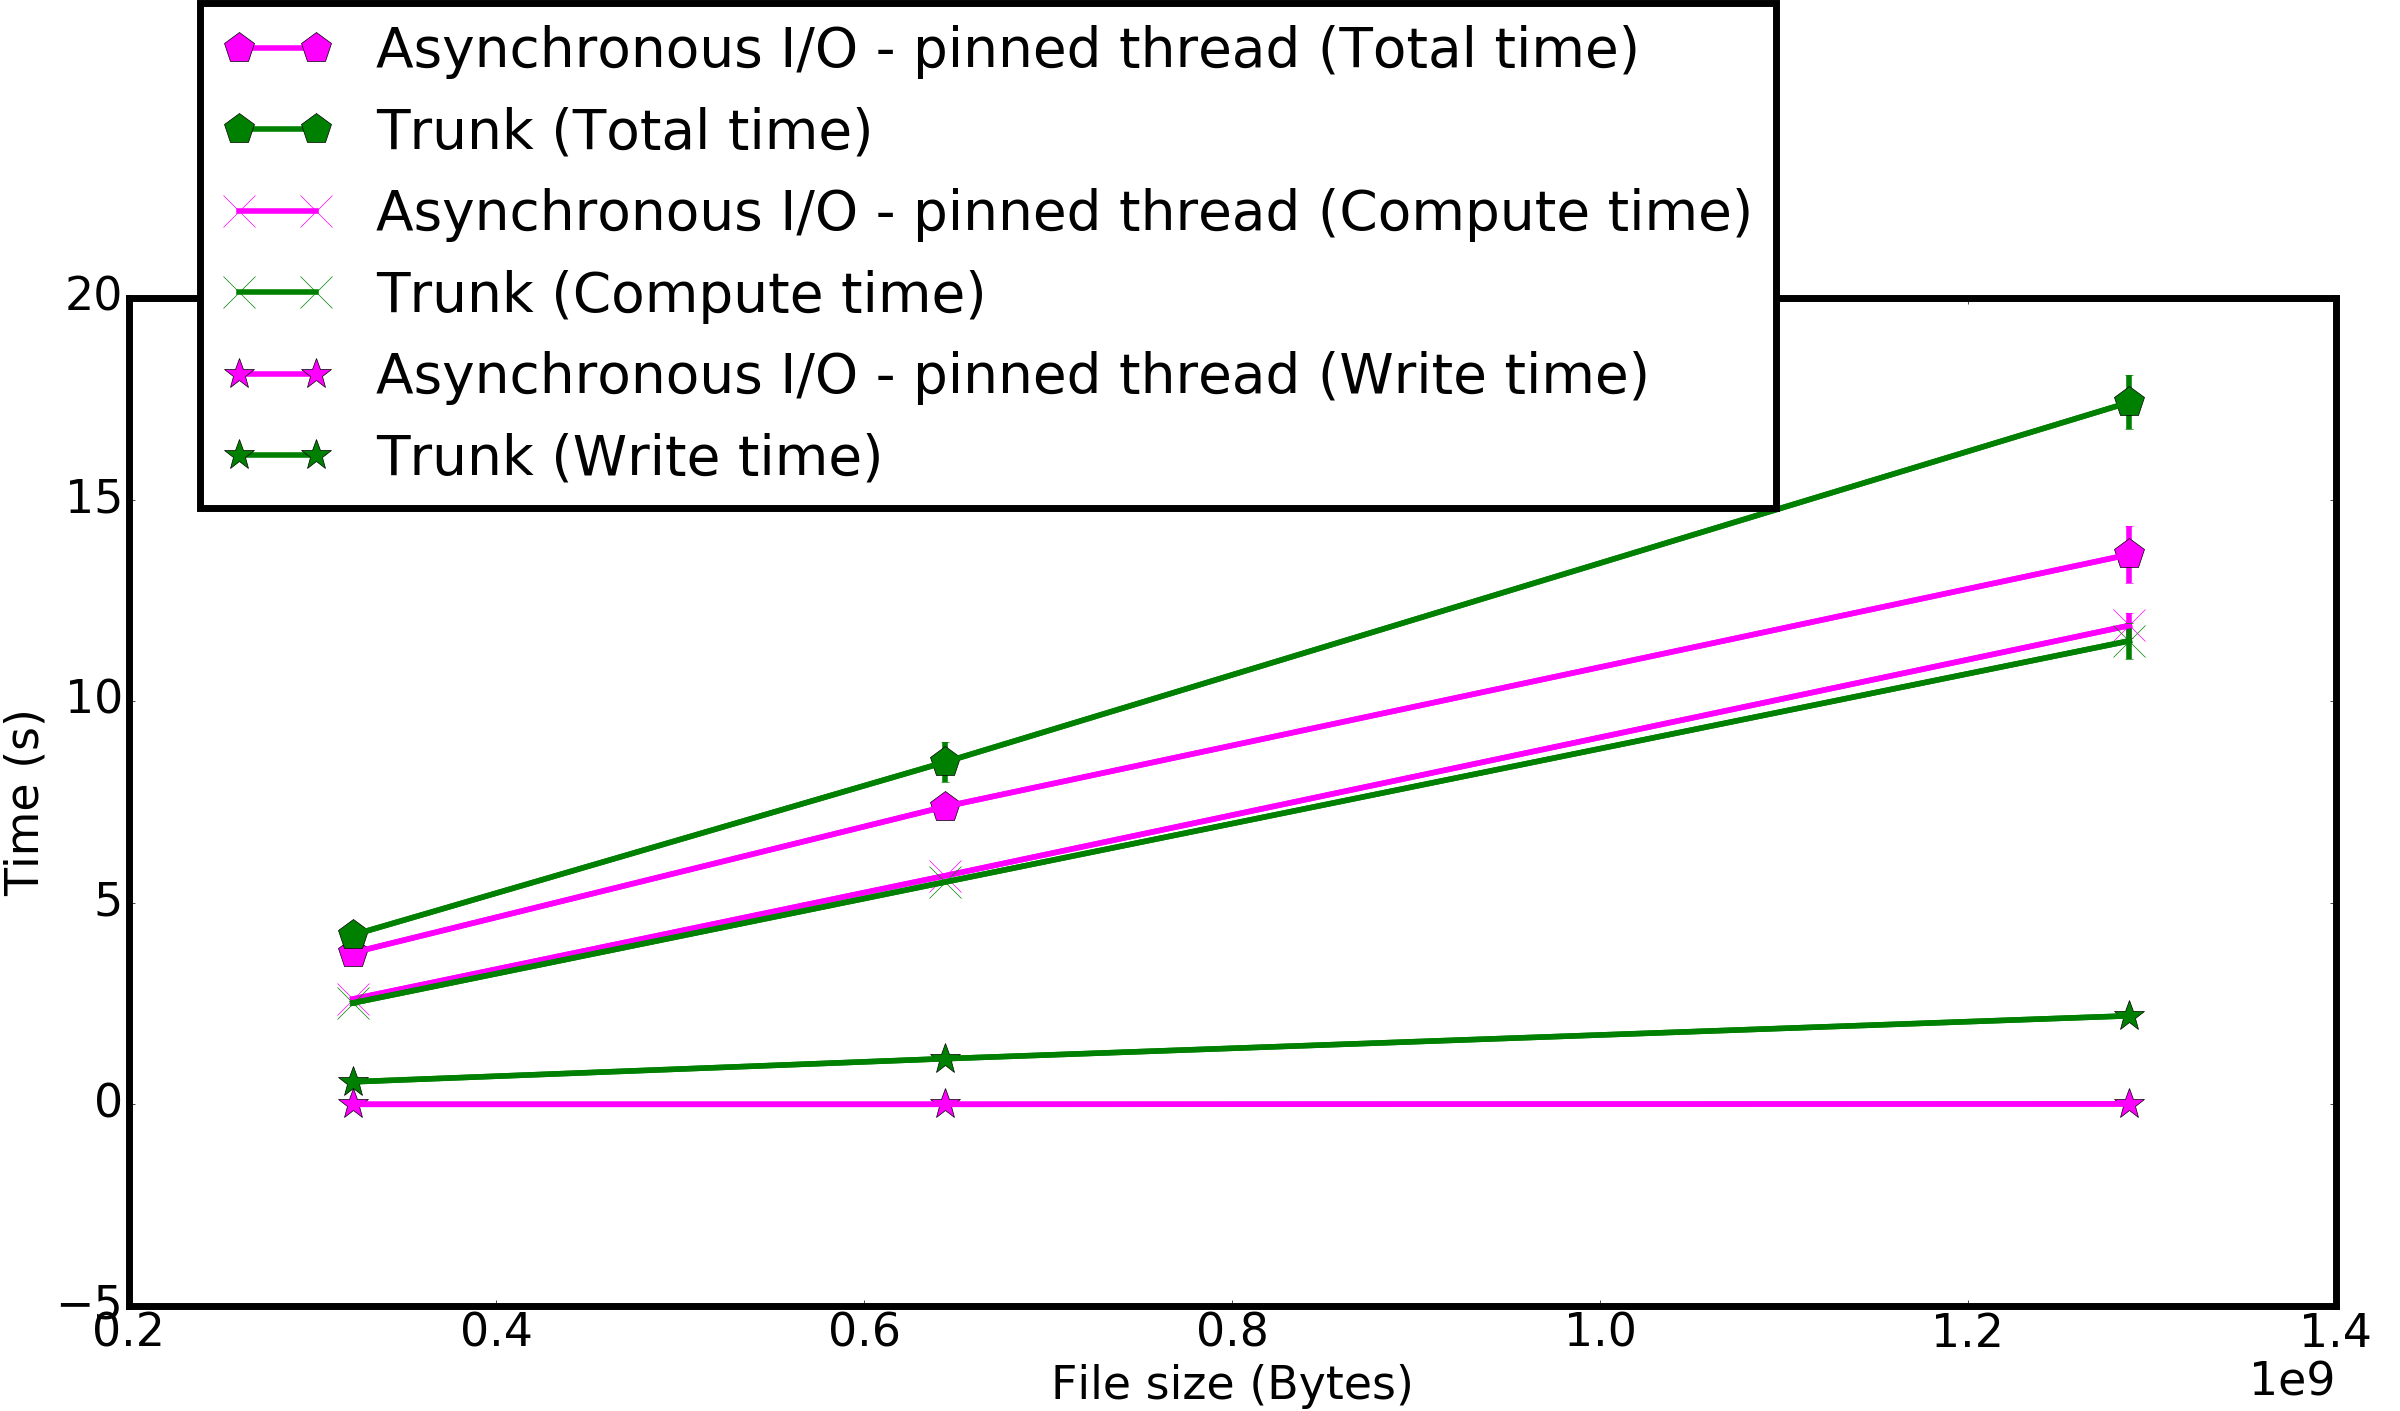
\includegraphics[width=\textwidth]{images/cubeRemapper_pthreadWrap_hpc.png}
				\end{subfigure}
			\end{figure}

			\begin{block}{}
			\begin{itemize}
				\item Lighten interference with \emph{"Compute"} thread
				\item Reduce \emph{"Compute"} time
			\end{itemize}
			\end{block}
		\end{frame}


% ----------------------------------------------------------------------------------------
		\begin{frame}
			\frametitle{False-sharing issue}
			\begin{figure}[!h]
				\centering
				\begin{subfigure}[b]{0.6\textwidth}
					\centering
					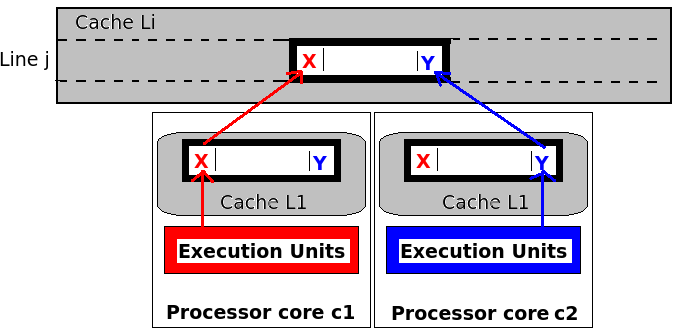
\includegraphics[width=\textwidth]{images/falseSharing_concecpt.png}
				\end{subfigure}
			\end{figure}

			\begin{block}{Consequence}
			\begin{itemize}
				\item Back and forth invalidation at each address access
				\item High occurrence frequency $\Rightarrow$ significant impact
			\end{itemize}
			\end{block}
		\end{frame}


% ----------------------------------------------------------------------------------------
		\begin{frame}
			\frametitle{Lighten the impact of false-sharing}
			\begin{figure}[!h]
				\centering
				\begin{subfigure}[b]{0.49\textwidth}
					\centering
					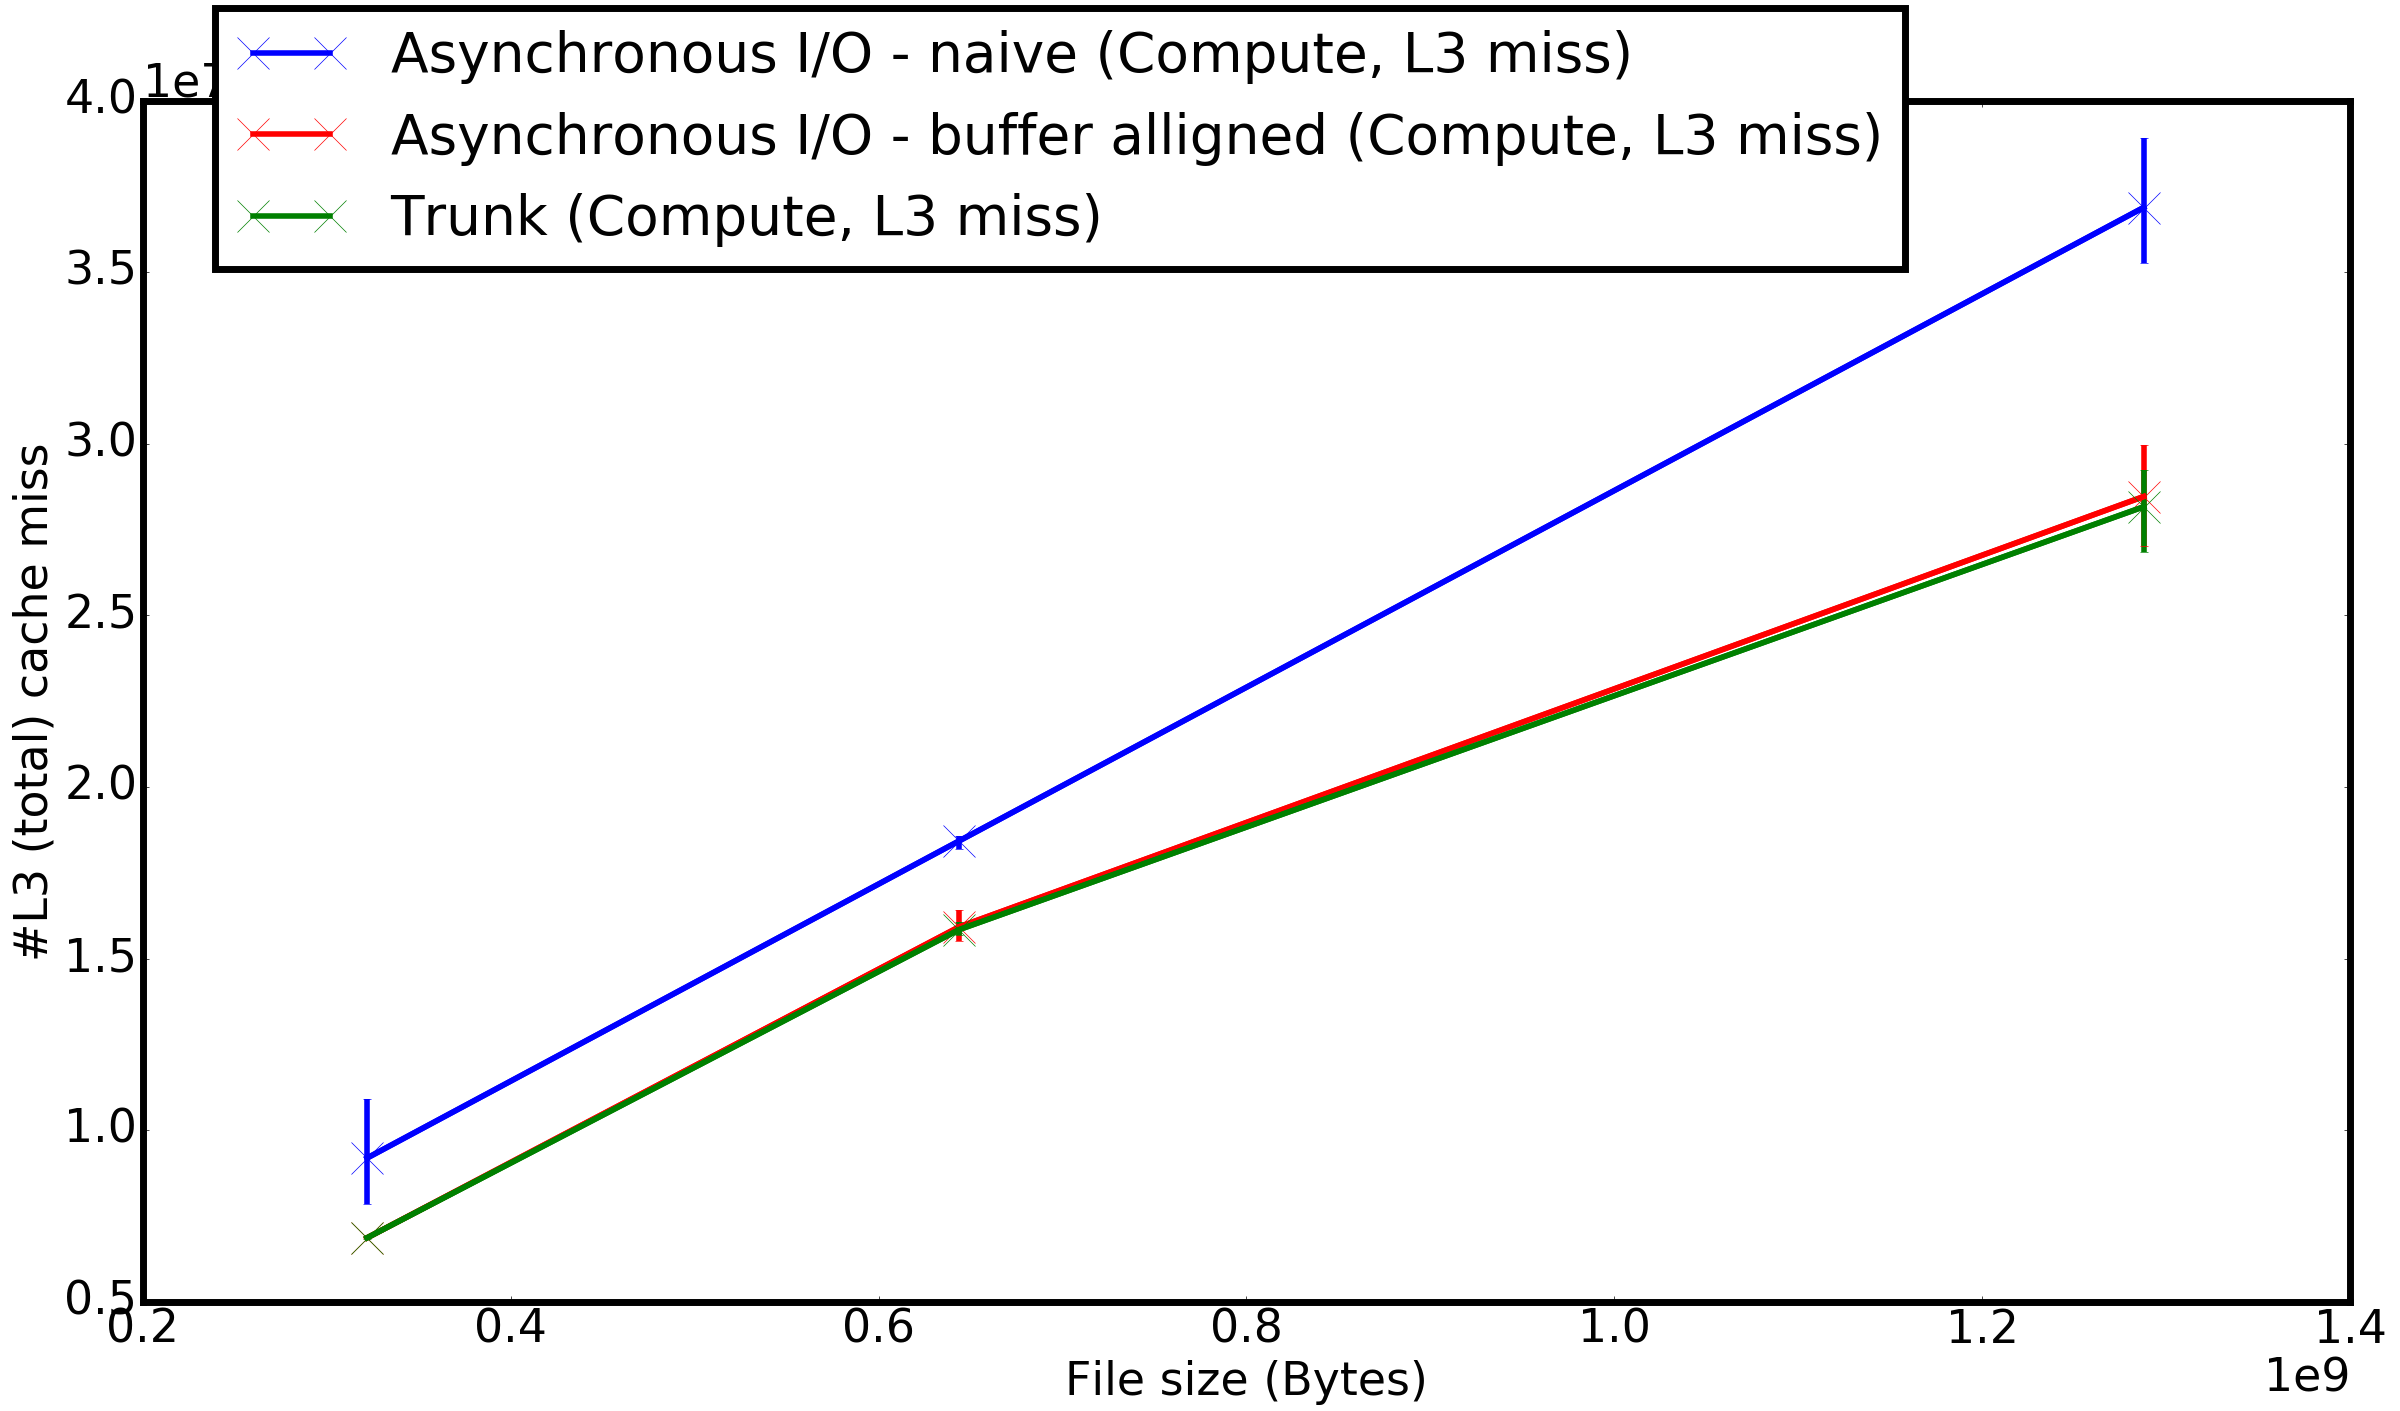
\includegraphics[width=\textwidth]{images/cubeRemapper_falseSharing_compute_trackL3_hpc.png}
					\caption[L3 (total) cache miss]%
					{{\small L3 (total) cache miss}}
				\end{subfigure}
				\hfill
				\begin{subfigure}[b]{0.49\textwidth}
					\centering
					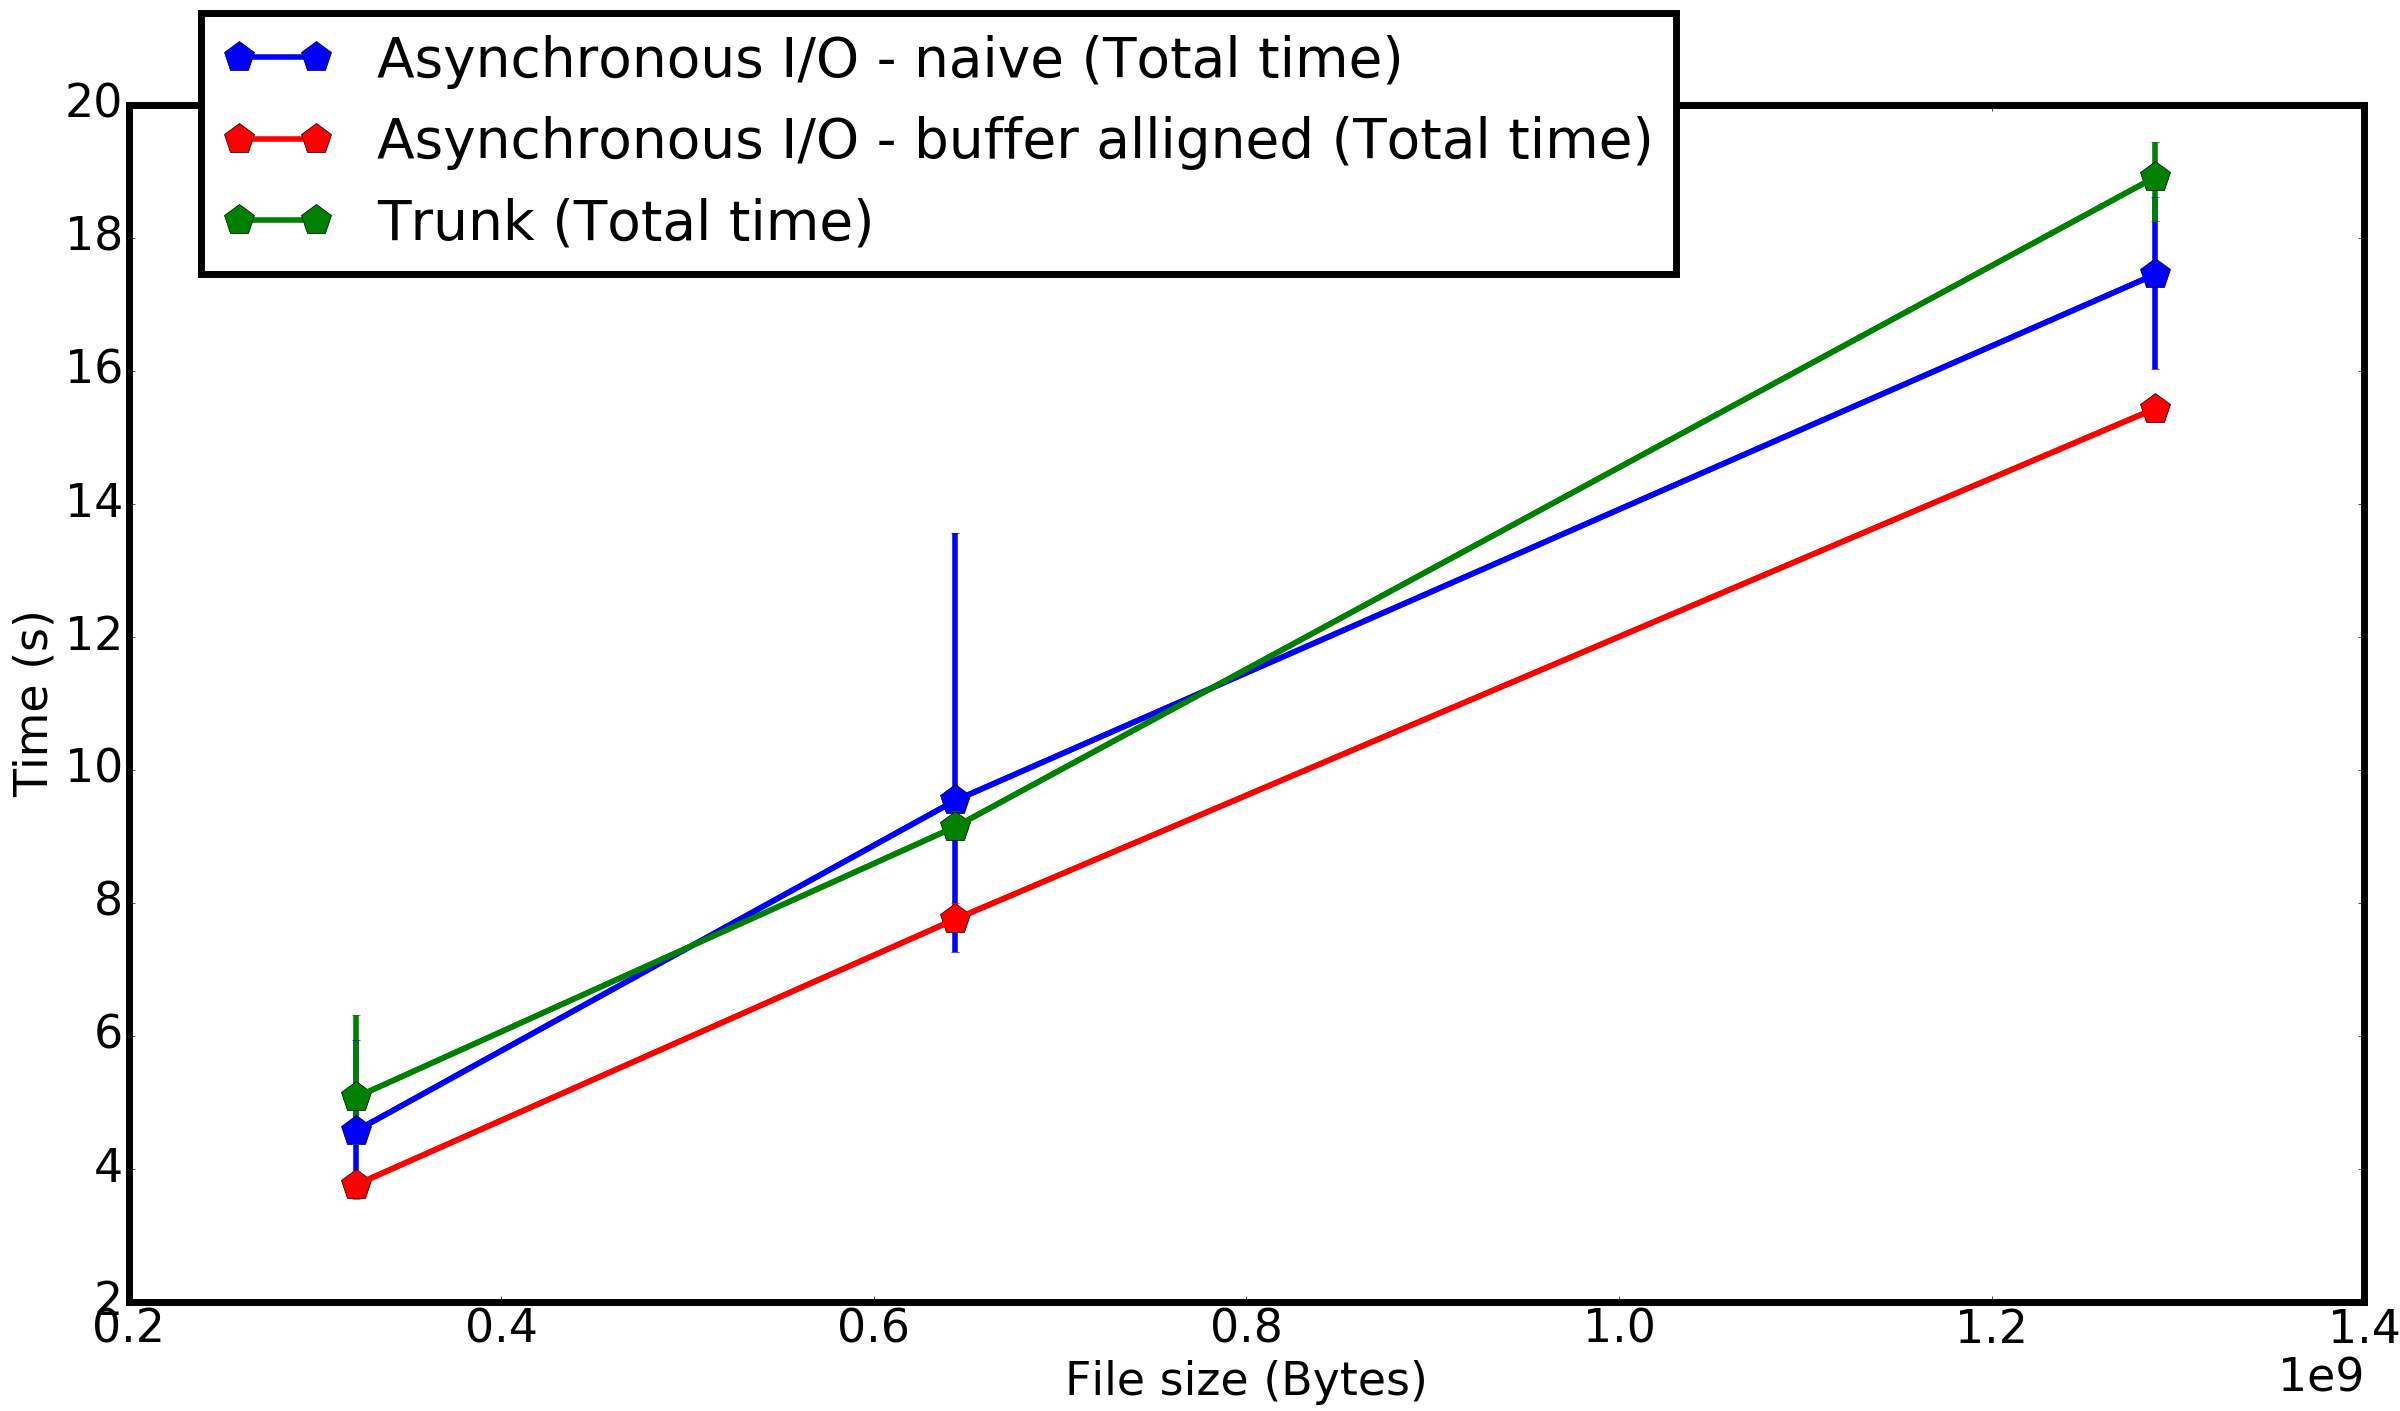
\includegraphics[width=\textwidth]{images/cubeRemapper_falseSharing_overall_time_hpc.png}
					\caption{\small \toolTargetSoftware\space \emph{"Total"} time}
				\end{subfigure}
			\end{figure}

			\begin{block}{}
			\begin{itemize}
				\pause
				\item Align buffer address to cache line
				\pause
				\item Reduce cache-miss rate
			\end{itemize}
			\end{block}
		\end{frame}


% ----------------------------------------------------------------------------------------
		\begin{frame}
			\frametitle{Improve dynamic memory allocation usage}
			\begin{figure}[!h]
				\centering
				\begin{subfigure}[b]{0.7\textwidth}
					\centering
					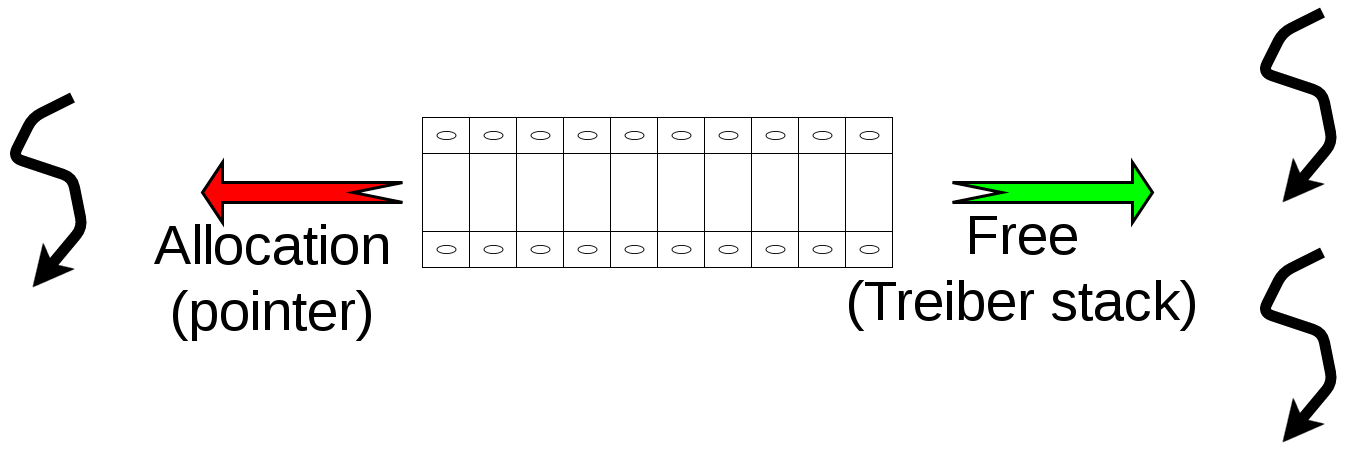
\includegraphics[width=\textwidth]{images/internship_juelich_customMemAlloc_freePool.png}
				\end{subfigure}
				\caption[Free dynamic memory pool]
				{\small Free dynamic memory pool}
			\end{figure}

			\begin{block}{Custom memory allocator}
			\begin{itemize}
				\item User-level managed heap
				\item Independent \emph{"allocation"} (Compute) and \emph{"free"} (Write)
				\item Reduced contention on "Free" pool (\emph{"Treiber"} stack)
			\end{itemize}
			\end{block}
		\end{frame}


% ----------------------------------------------------------------------------------------
		\begin{frame}
			\frametitle{Improve dynamic memory allocation usage}
			\begin{figure}[!h]
				\centering
				\begin{subfigure}[b]{0.8\textwidth}
					\centering
					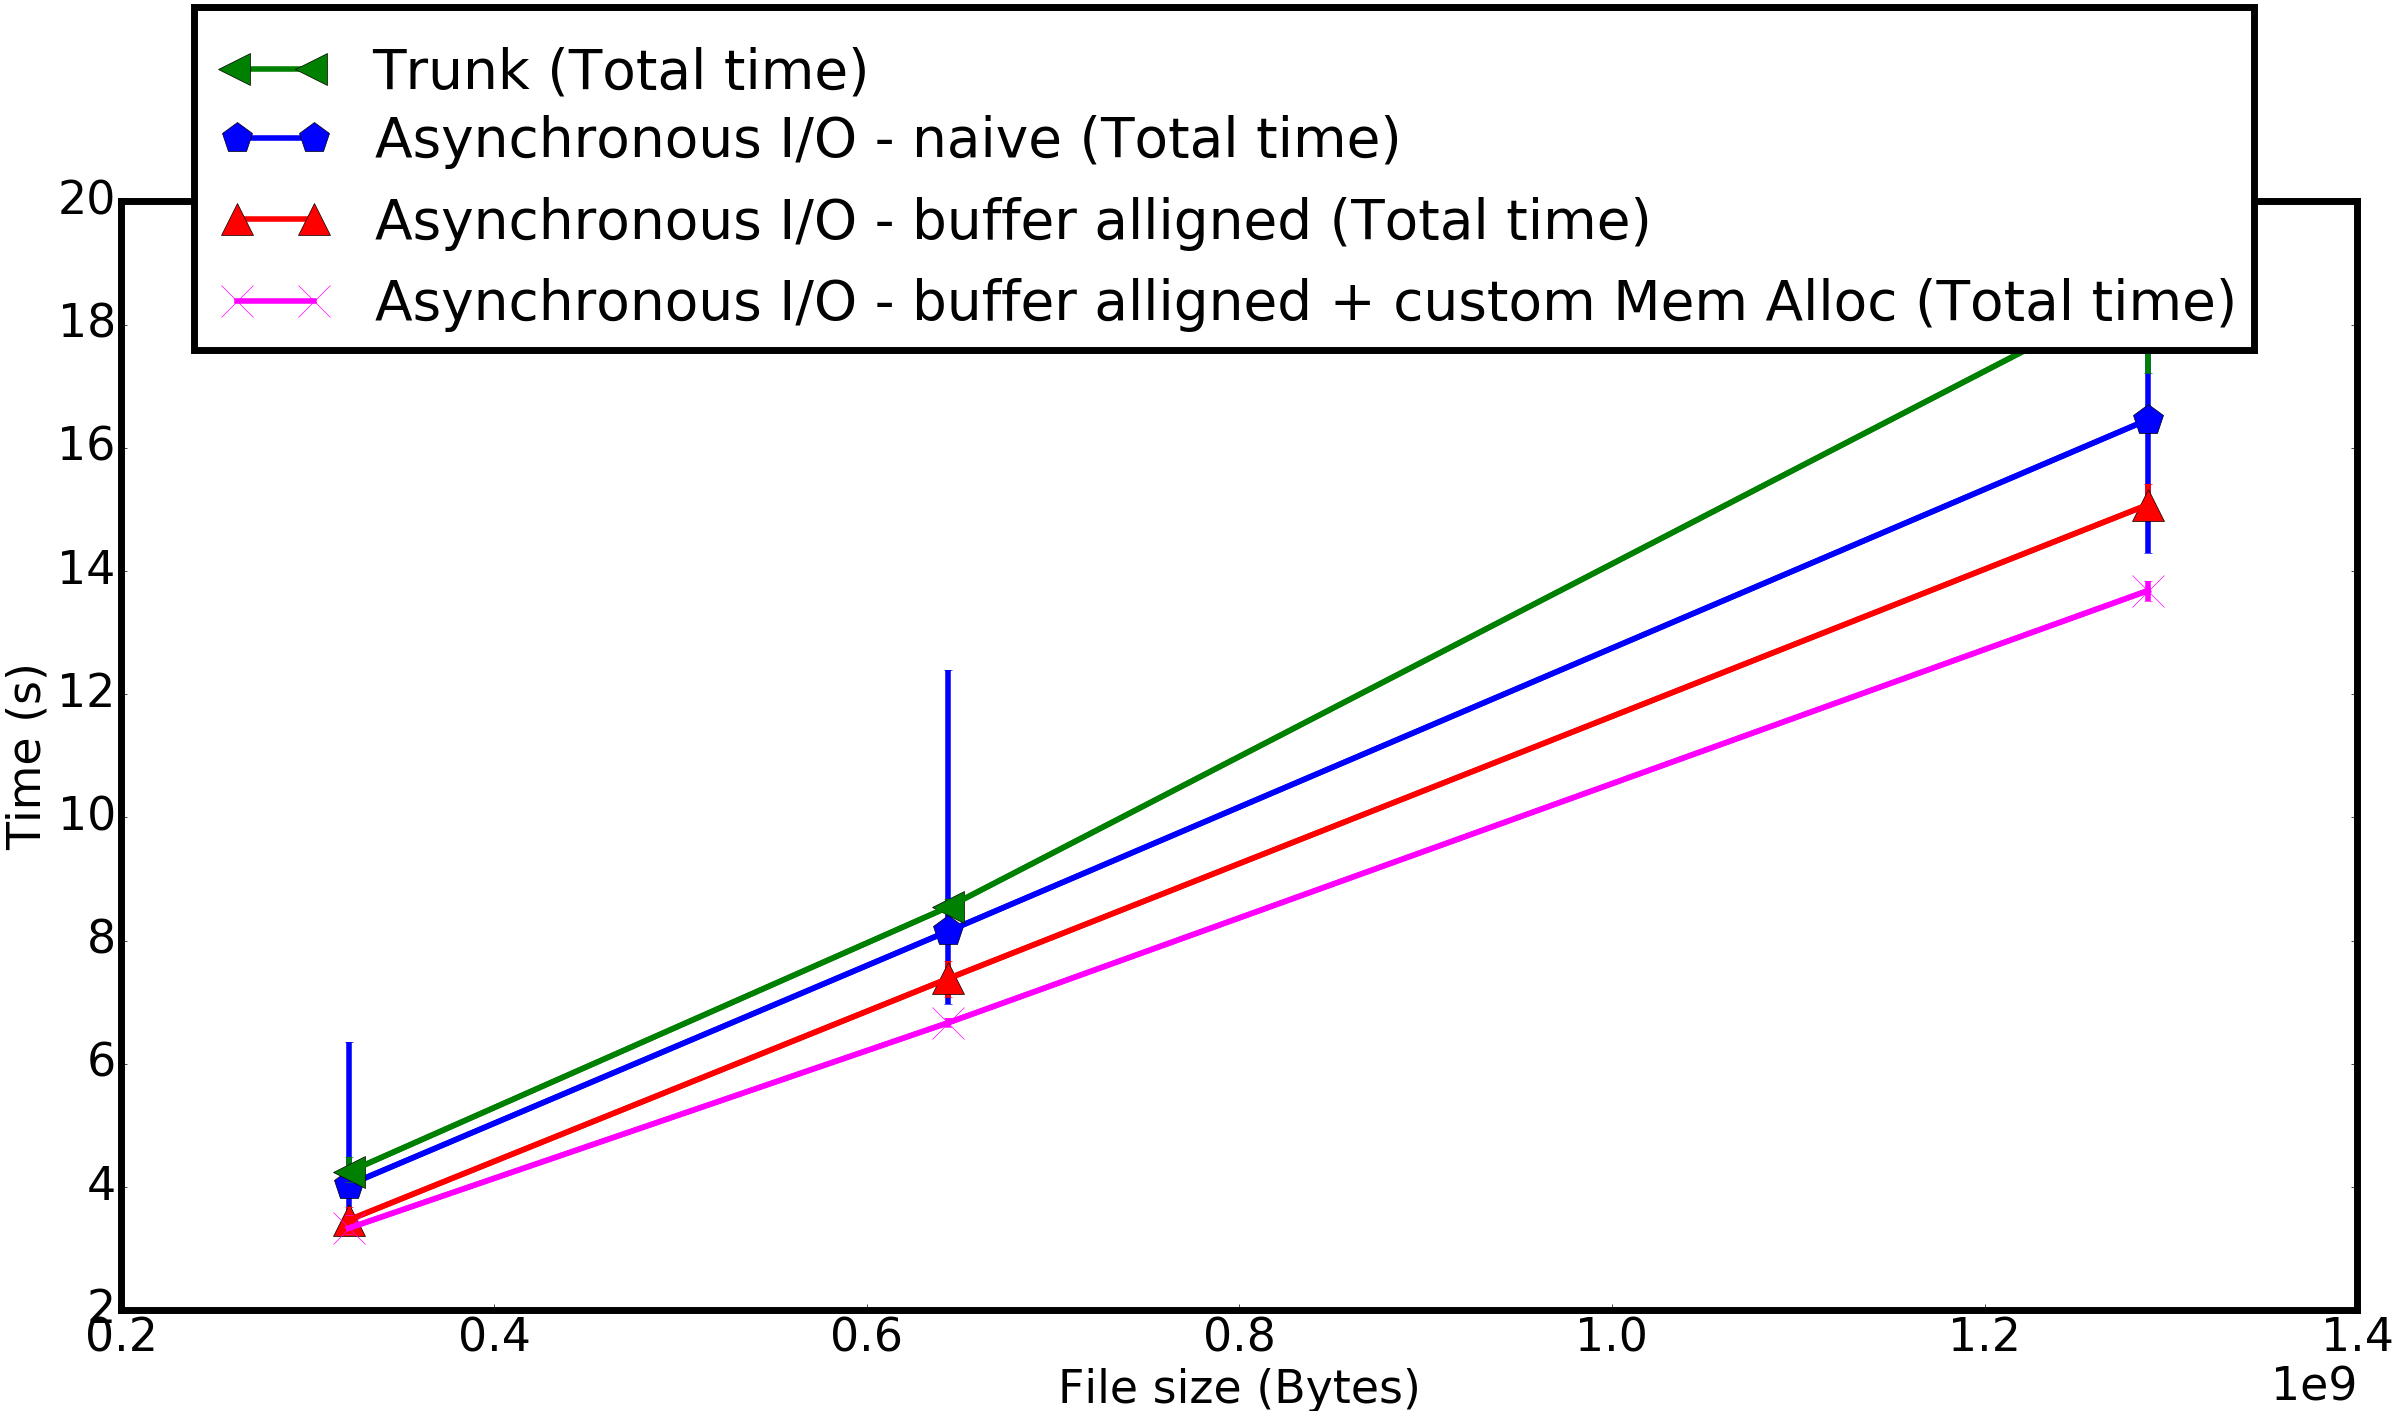
\includegraphics[width=\textwidth]{images/cubeRemapper_customMemAlloc_overall_time_hpc.png}
				\end{subfigure}
				\caption{\toolTargetSoftware\space full-fledged assessment}
			\end{figure}
		\end{frame}


% ----------------------------------------------------------------------------------------
\section{Conclusion and future work}
	\begin{frame}[c]{Conclusion}
		\begin{itemize}
			\item Studied theoretical model of \notationaio\space (AIO) within the \toolTargetSoftware\space pattern
			\pause
			\item Implemented prototype version (candidate for production) of the \toolTargetSoftware\space
			\pause
			\begin{itemize}
				\item Identified runtime perturbation created by AIO
				\item Suggested and evaluated solutions
			\end{itemize}
		\end{itemize}

		\pause
		Our most enhanced custom implementation of the \toolTargetSoftware\space allows a significant improvement
	\end{frame}


% ----------------------------------------------------------------------------------------
	\begin{frame}[c]{Future work}
		Full parallelization of the pattern:
		\begin{itemize}
			\item Multiple concurrent \emph{"compute"} threads
			\item Expected fit with our current solution:
			\begin{itemize}
				\item Optimal data distribution/synchronization
				\item Allows further scalability evaluation of current solution
			\end{itemize}
		\end{itemize}
	\end{frame}


% ----------------------------------------------------------------------------------------
\begin{frame}
\vspace{1cm} 
\begin{center}
\huge{\textbf{Thanks for your attention!}}
\end{center}
\end{frame}





	



\end{document}



